
\section{Frequency control} \label {sec: controle_freq}

In modern systems, control over the processor frequency can be done by hardware with independent circuits as well as by software. For that, there is the Advanced Configuration and Power Interface (ACPI) an open standard adopted by operating systems to configure hardware components related to power management.

In the ACPI two important states for the DVFS are defined that optimize the energy consumption. They are "C", which is activated when the processor is not executing any instructions, and "P", which is activated while the processor is operating. These states have several levels and at each level the frequency and voltage are changed.

State P starts at level P0, where frequency and voltage are the maximum possible, then P1, where both decrease, until reaching the last state, Pn, where frequency and voltage are the lowest possible. The change of state depends on the level of utilization of the processor. To stay in each state, the level of processor usage must be within specific limits. After exceeding these limits for a certain time, the state will change to the next state corresponding to that new level of processor usage. The number of possible states depends on each manufacturer.

After an idle time, the processor begins to activate C states, starting with C0 where it is still fully active, then moving to C1, where some features are disabled, up to Cn, where all possible features are disabled. The ACPI standard establishes the functionalities that can be disabled between level C1 and level C3, as seen in Table \ref {tab: states_c}. The other levels are specific to each manufacturer.

\begin {table} [H]
\centering
\begin {tabular} {| l | l | l |}
\hline
Mode & Name & Functionality \\ \hline
C0 & operating state & Active processor \\ \hline
C1 & Halt & Stop executing instructions \\ \hline
C2 & Stop-Clock & Disable the internal clock \\ \hline
C3 & Sleep & Disable cache coherence \\ \hline
\end {tabular}
\caption {C states}
\label {tab: states_c}
\end {table}

In state C, the higher the level the greater the energy savings, but returning to the fully functional level is more difficult. In states P, there is a trade-off between performance and energy savings. Figure \ref {fig: p_state} best illustrates the change of states, in which we can see which parts of the circuits are deactivated in states C, the latency to return to the active state, power consumption and also shows the relationship of states P with often.

\begin {figure} [H]
\centering
\begin{subfigure}[t]{0.5\textwidth}
\centering
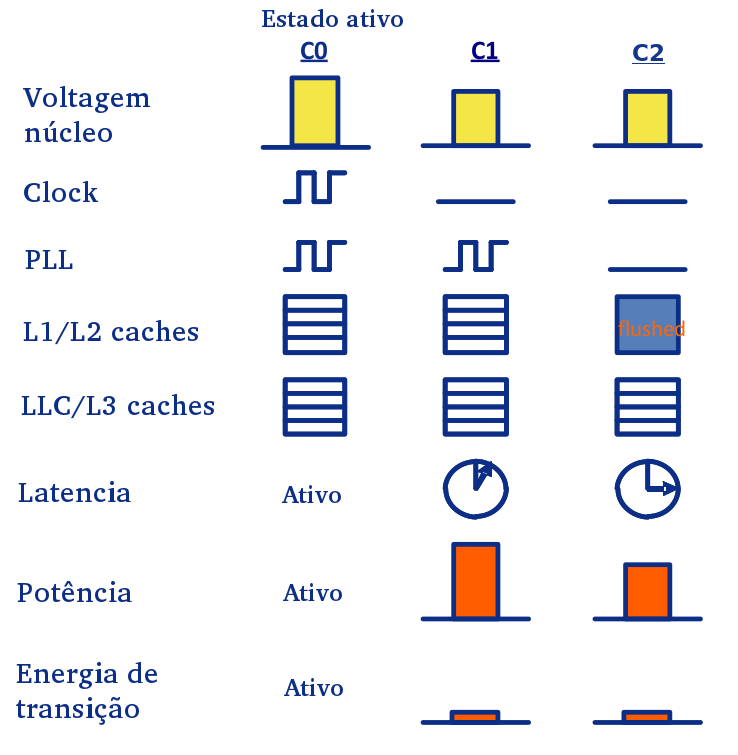
\includegraphics[height= 7.5cm]{intro/figures/c_states}
\caption {C states}
\end {subfigure}%
~
\begin{subfigure}[t]{0.5\textwidth}
\centering
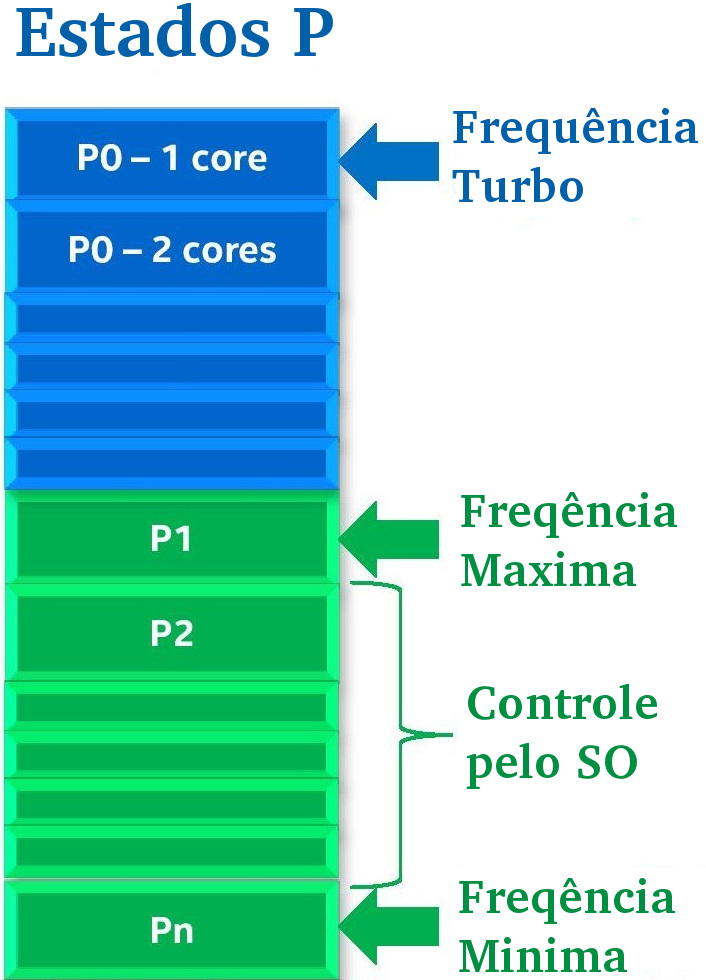
\includegraphics[height= 7.5cm]{intro/figures/p_states}
\caption {States P}
\end {subfigure}
\caption {Illustration of states C and P} {Altered image from \protect \url {https://www.thomas-krenn.com/en/wiki/Processor_P-states_and_C-states}}
\label {fig: p_state}
\end {figure}


% Are states C and P orthogonal, do they operate independently?

For this management, the operating system provides in the user space a way to control the frequency. This work used an operating system that has Linux as its core.

Linux is compatible with several modern architectures and is widely used in servers, smartphones and supercomputers. It was based on the UNIX system which has the philosophy of treating everything on the system as a file, including settings and input and output devices, such as keyboard, mouse and hard drive. Another important feature is that it is modular and parts of the system can be loaded or removed during execution.

On Linux there are several frequency management options \cite {Brown2005}. The main ones are acpi-cpufreq, Intel P-state, AMD powernow. In this work, acpi-cpufreq is used, which is standard and allows direct control of frequency through system files. Acpi-cpufreq is a Linux module that uses implemented policies that dynamically decide the frequency to be used. Some of these policies are:

\begin {itemize}
\item Performance - configured as often as possible
\item Powersave - configured as low as possible
\item Userspace - the user chooses the frequency to be used
\item Ondemand - controls the frequency depending on the processor load. When the load increases the frequency also increases accordingly.
\item Conservative - similar to Ondemand but more smoothly, the frequency increase is continuous instead of jumping.
\end {itemize}

\section {Power consumption monitoring} \label {sec: monitoring}
The Running Average Power Limit (RAPL) and Intelligent Platform Management Interface (IPMI) interfaces were used to measure the power consumed. described in \cite{November2013}.

\subsection {IPMI}
IPMI \cite {November2013} is a set of specifications for autonomous subsystems that provides processor, firmware and operating system independent management and monitoring. The use of IPMI allows system administrators to avoid having to travel to the server location, which is often far away, to perform their tasks. Also, servers are located in places with low temperature and with a lot of noise due to the ventilation system, and one should avoid spending too much time in these places. With remote management, it is possible to turn the system on and off, remotely access the (BIOS) and reinstall the system in case of any serious failure.

\begin {figure} [H]
\centering
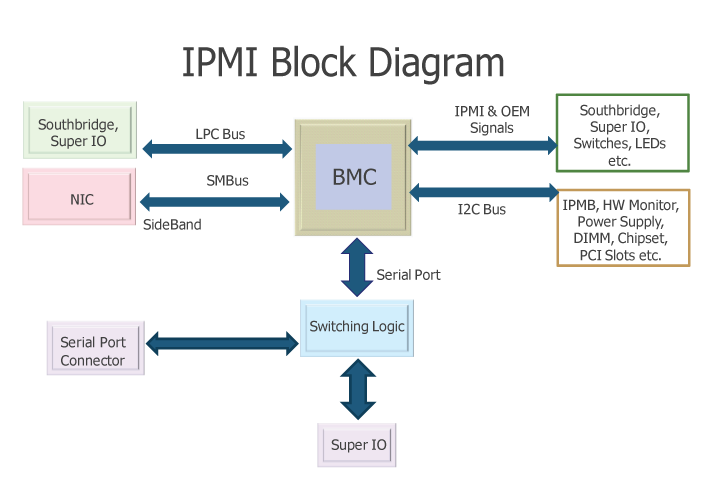
\includegraphics [height = 7.5cm] {intro/figures/IPMI-Block-Diagram.png}
\caption {IMPI diagram} {Image taken from \protect \url {https://pt.wikipedia.org/wiki/Intelligent_Platform_Management_Interface}, the main components of IPMI and how they communicate are shown}
\label {fig: IPMI}
\end {figure}

Access to the IPMI network can be done using the HTTP protocol or a tool made available by the manufacturer (ipmitool), which also performs access via the network. It is also used to monitor the status of the platform with a set of sensors coupled with system temperatures, voltages, fans and power supplies.

\subsection {RAPL}

Modern Intel microprocessors, based on the SandyBridge architecture, include the RAPL \cite {Rotem2012, Hahnel2012, Hackenberg2015} interface designed to limit the use of energy on a chip while ensuring maximum performance. This interface supports energy measurement capabilities through an integrated circuit that estimates energy use based on a model driven by architectural event counters for all components. It also provides temperature readings and current leak models. Estimates are made available in model-specific registers (MSR), updated in milliseconds. The energy estimates offered by RAPL were validated by Intel, which showed excellent results.


\section{Verifying models hypothesis}

\subsection{Frequency voltage ratio}

\begin{table}[H]
	\begin{tabular}{|c|c|c|c|c|c|c|c|c|c|c|c|}
		\hline
		Freq (GHz) & 2.2   & 2.1   & 2.0   & 1.9   & 1.8   & 1.7   & 1.6   & 1.5   & 1.4   & 1.3   & 1.2   \\ \hline
		V          & 0.77  & 0.76  & 0.75  & 0.74  & 0.73  & 0.72  & 0.71  & 0.70  & 0.69  & 0.68  & 0.67  \\ \hline
		aperf      & 2.199 & 2.099 & 2.000 & 1.899 & 1.799 & 1.699 & 1.599 & 1.500 & 1.397 & 1.297 & 1.200 \\ \hline
	\end{tabular}
\end{table}

\begin{figure}[H]
	\centering
	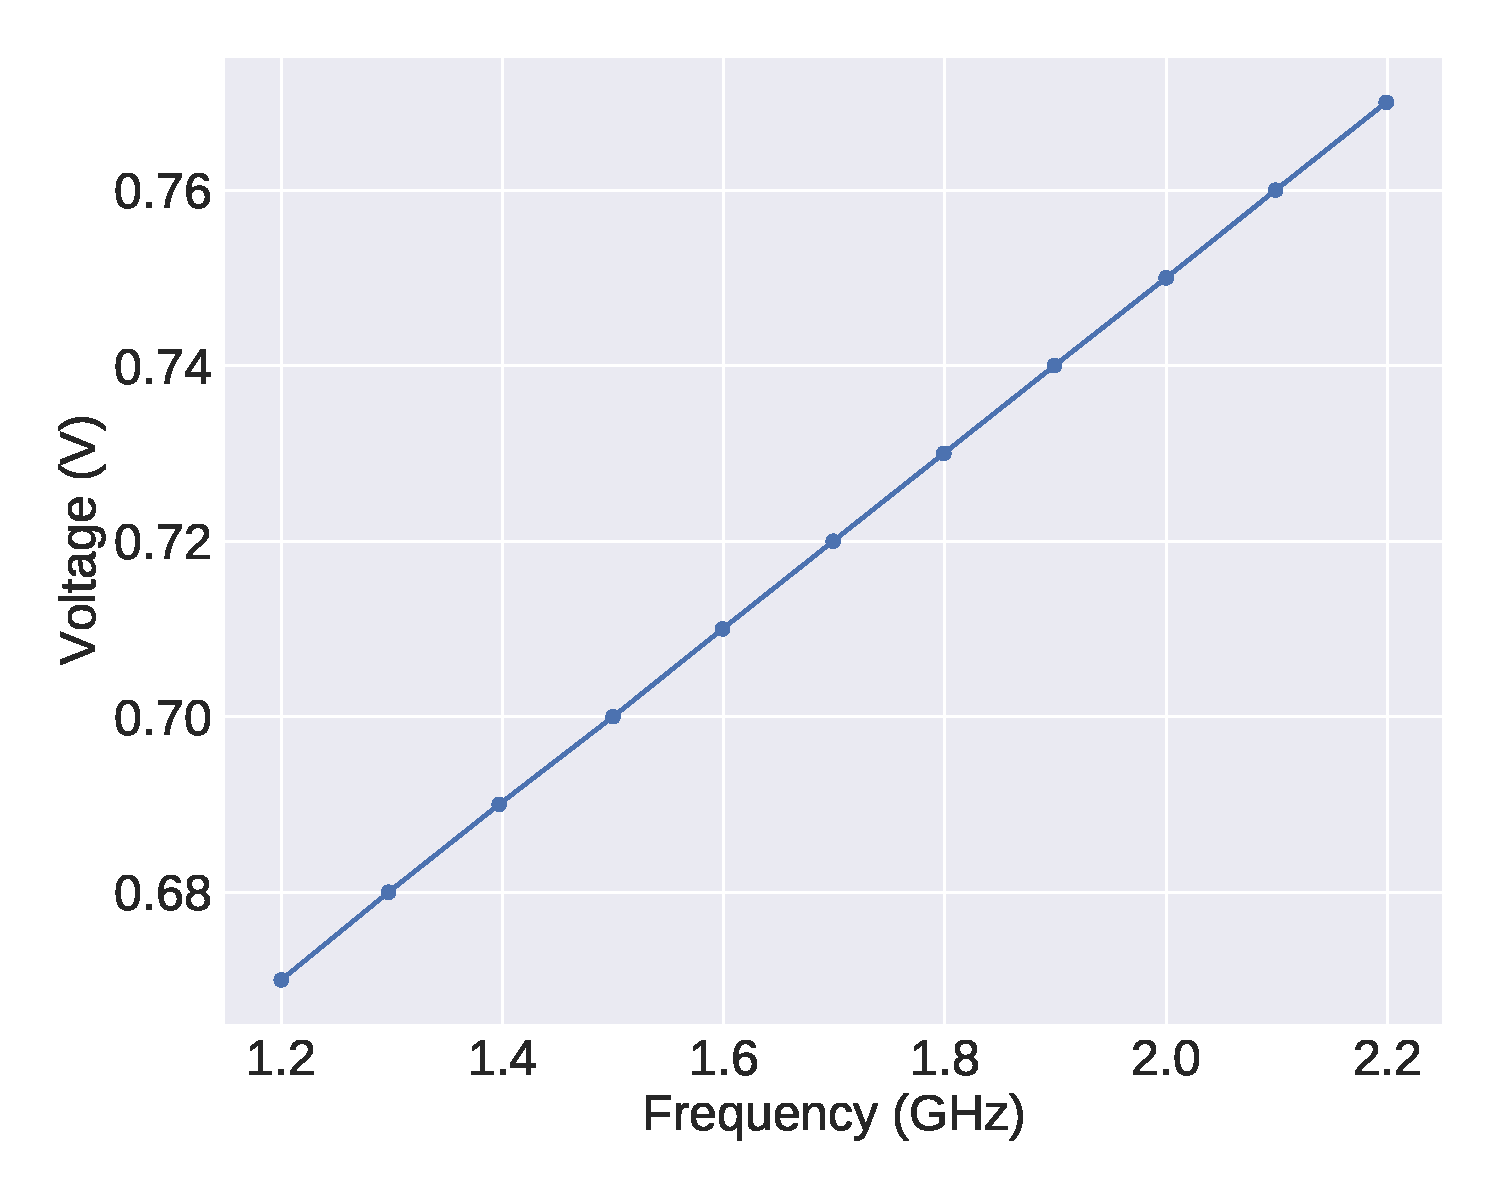
\includegraphics[width=\columnwidth]{experiments/figures/freq_volt_rel.png}
	\caption{Frequency voltage relation}
	\label{fig:freq_volt_rel}
\end{figure}

\subsection{Instructions executed}

\begin{table}[H]
	\caption{Cores variation}
	\begin{tabular}{|c|c|c|c|}
		\hline
		Application  & Instructions & Dev.     & Dev. (\%) \\ \hline
		Vip          & 7.97e+11     & 7.16e+06 & 0.00\%    \\ \hline
		Openmc       & 8.17e+07     & 1.65e+04 & 0.02\%    \\ \hline
		Rtview       & 9.91e+12     & 1.55e+09 & 0.02\%    \\ \hline
		X264         & 4.52e+11     & 5.81e+07 & 0.01\%    \\ \hline
		Bodytrack    & 1.86e+12     & 3.95e+10 & 2.13\%    \\ \hline
		Fluidanimate & 2.09e+12     & 8.44e+10 & 4.04\%    \\ \hline
		Xhpl         & 1.14e+08     & 1.24e+05 & 0.11\%    \\ \hline
		Blackschole  & 3.75e+12     & 1.40e+09 & 0.04\%    \\ \hline
		Dedup        & 1.02e+11     & 5.74e+07 & 0.06\%    \\ \hline
		Swapti       & 2.43e+12     & 8.87e+08 & 0.04\%    \\ \hline
		Canneal      & 1.19e+11     & 4.46e+07 & 0.04\%    \\ \hline
		Freqmine     & 1.27e+12     & 4.78e+08 & 0.04\%    \\ \hline
		Ferret       & 4.76e+11     & 7.04e+07 & 0.01\%    \\ \hline
	\end{tabular}
\end{table}

\begin{table}[H]
	\caption{Frequency Variation}
	\begin{tabular}{|c|c|c|c|}
		\hline
		Application  & Instructions & Dev.     & Dev. (\%) \\ \hline
		Vip          & 7.97e+11     & 1.16e+06 & 0.00\%    \\ \hline
		Openmc       & 8.17e+07     & 4.52e+03 & 0.01\%    \\ \hline
		Rtview       & 9.91e+12     & 6.64e+05 & 0.00\%    \\ \hline
		X264         & 4.52e+11     & 1.54e+05 & 0.00\%    \\ \hline
		Bodytrack    & 1.84e+12     & 2.54e+05 & 0.00\%    \\ \hline
		Fluidanimate & 2.38e+12     & 1.70e+09 & 0.07\%    \\ \hline
		Xhpl         & 1.14e+08     & 5.95e+03 & 0.01\%    \\ \hline
		Blackschole  & 3.75e+12     & 4.36e+05 & 0.00\%    \\ \hline
		Dedup        & 1.02e+11     & 8.32e+07 & 0.08\%    \\ \hline
		Swapti       & 2.43e+12     & 1.48e+05 & 0.00\%    \\ \hline
		Canneal      & 1.19e+11     & 3.01e+05 & 0.00\%    \\ \hline
		Freqmine     & 1.27e+12     & 3.70e+08 & 0.03\%    \\ \hline
		Ferret       & 4.76e+11     & 5.63e+07 & 0.01\%    \\ \hline
	\end{tabular}
\end{table}

\subsection{Input size and instructions}

\begin{figure}[H]
	\centering
	\includegraphics[width=\columnwidth]{models/figures/hypothesis/input_instructions/fp/blackscholes.png}
	\caption{Caption}
	\label{fig:my_label}
\end{figure}

\begin{figure}[H]
	\centering
	\includegraphics[width=\columnwidth]{models/figures/hypothesis/input_instructions/fp/canneal.png}
	\caption{Caption}
	\label{fig:my_label}
\end{figure}

\begin{figure}[H]
	\centering
	\includegraphics[width=\columnwidth]{models/figures/hypothesis/input_instructions/input_time/blackscholes.png}
	\caption{Caption}
	\label{fig:my_label}
\end{figure}

\begin{figure}[H]
	\centering
	\includegraphics[width=\columnwidth]{models/figures/hypothesis/input_instructions/input_time/canneal.png}
	\caption{Caption}
	\label{fig:my_label}
\end{figure}

\section{Model experimental validation} \label{sec:experimentalvalidation}
In this section, the models presented in~\cref{sec:powermodel} and~\cref{sec:performancemodel} were validated with a benchmark specific for multi-core architectures. Additionally, in order to assess the modeling overhead and accuracy, our proposal was then compared to machine learning approaches. We compared against Support Vector Regression (SVR)~\cite{Smola2004}, Decision Tree \cite{Kitts2006RegressionLecture}, k-nearest neighbors \cite{Altman1992AnRegression}, Multilayer perceptron \cite{Murtagh1991MultilayerRegression}, and some new methods such as Gao et al. \cite{Gao2019DendriticPrediction}. However, SVR was chosen as the most representative because in our tests it performed best without an aggressive fine-tuning.

\subsection{Case-Study Applications} \label{sec:casestudyapplication}
The PARSEC parallel benchmark suite, version 3.0~\cite{Bienia2008}, OpenMC \cite{Romano2015OpenMC:Development} and LINPACK (HPL) \cite{Dongarra1988TheExplanation}, were chosen as case studies. The PARSEC benchmark focused on emerging workloads and was designed to represent the next-generation shared-memory programs for chip-multiprocessors. It covers an ample range of areas such as financial analysis, computer vision, engineering, enterprise storage, animation, similarity search, data mining, machine learning, and media processing. The OpenMC and the LINPACK are two classic HPC programs.

\subsection{Case-Study Architecture} \label{sec:casestudyarchitecture}
The experiments were executed in one computer node equipped with two Intel Xeon E5-2698 v3 processors with sixteen cores each and two hardware threads for each core. The overall view of the architecture is shown in Figure \ref{fig:architecture}. The maximum non-turbo frequency is 2.3GHz, and the total physical memory of the node is 128GB (8$\times$16GB). Turbo frequency and hardware multi-threading were disabled during all experiments. The operating system used was Linux CentOS 6.5, kernel 4.16. 

\begin{figure}[htb!]
	\centering
	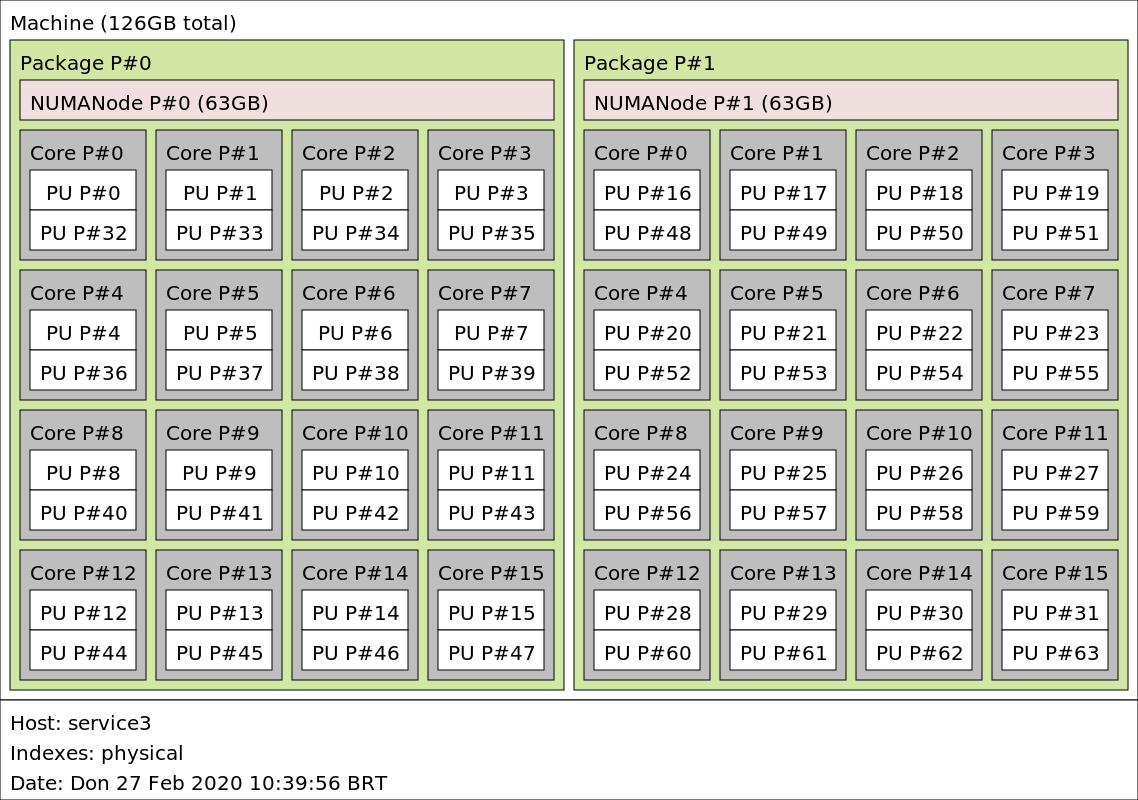
\includegraphics[width=\columnwidth]{models/figures/architecture.png}
	\caption{Node architecture (the image was made with the lstop application).}
	\label{fig:architecture}
\end{figure}

The Linux kernel has many different policies for power management, depending on the driver. In the default driver, the acpi-cpufreq, the options are:
\begin{itemize}
	\item Powersave
	\item Performance
	\item Ondemand
	\item Conservative
	\item Userspace
\end{itemize}
In this work, the frequency control was performed using the Userspace governor, and the core control was accomplished by modifying the appropriate system files with the default CPU-hotplug driver.

The architecture is equipped with the Intelligent Platform Management Interface (IPMI), a set of interfaces allowing out-of-band management of computer systems and platform-status monitoring via the local network~\cite{Schwenkler2006IntelligentInterface}. It can monitor variables and resources such as the system's temperature, voltage, fans, and power supplies, with independent sensors attached to the hardware.

\subsection{Fitting the Models} \label{sec:fitting}
To find the parameters of the \cref{eq:en_final}, 10 uniformly random configurations of frequencies ($f$), cores ($p$) and inputs ($N$) were chosen from the range $1<=p<=32$, $1.2<=f<=2.2$ and $1<=N<=5$ respectively. The application was executed for each chosen configuration, and the measured  energy and time values were collected. For the input size if we assume that all CPU instructions are executed at approximately the same time, the number of basic operations will be directly correlated with the time. Thus, we can estimate the problem size by looking at the execution time, allowing us to divide a large problem size into several smaller ones knowing their relationship as done in the work of Oliveira ~\cite{Oliveira2018ApplicationCores}. The unity can also vary depending on the definition. In our case for simplicity, we assign numbers from 1 the smallest size to 10 the largest, increasing the problem linearly, that way its also possible to interpolate any input in between these values.

%The application's input was chosen to increase the workload linearly, from smallest to largest, so that most of the input space is covered~\cite{Oliveira2018ApplicationCores}. 

For each configuration, samples of the power were collected using IPMI every 1 second. This sampling rate was chosen because the order of magnitude of the mean run time of the applications is minutes. Therefore, this rate provides enough samples to measure average power. Additionally, timestamps and the total run time were collected. The total energy spent on each configuration is estimated by first interpolation the power samples using a first order method and then integrating this function in the time.

From the sampled data, the parameters of the model can be estimated. This results in an optimization problem of finding the parameters that minimize the distance between estimated and the measured values. To solve this minimization problem, non-linear least squares have been applied. 

The python library scikit-learning was used to build the SVR model~\cite{PedregosaFandVaroquauxGandGramfortAandMichel2011Scikit-learn:Python}. The SVR was trained using the same data used for parameters estimation of \cref{eq:en_final} with a grid search used to find the best kernel function and the best values for the hyper-parameters penalty for the wrong ($C$) and ($\gamma$). For this data, the best function was the Radial Base Function (RBF), and the hyper-parameters were $C=10^4$ and $\gamma=0.5$. 

\subsection{Measured versus Modeled Energy}
\label{sec:measuredversusmodeledenergy}

To validate the proposed energy model, all possible configurations were tested by varying the cores in a range of $1<=p<=32$, the frequency in $1.2<=f<=2.2$ and the input in $1<=N<=5$, which varies from 400 to over 1000 configurations depending on the application as some applications have restrictions on the number of cores. The mean percentage error was computed as the difference between the estimated and measured values according to the following equation:
\begin{equation}
MPE = \frac{1}{N} \sum_i^N \frac{|y_{\rm estimated}-y_{\rm measured}|}{y_{\rm measured}}.
\label{eq:mpe}
\end{equation}

\subsubsection{Frequency x Cores}
Figures \ref{fig:en_eq_black}, \ref{fig:en_eq_canneal} plot the measured and modeled energy consumption for some of the applications modeled. They  show some of the possible shapes that the model can take while varying the number of active cores, operating frequency, and input size.
\begin{figure}[H]
	\centering
	\begin{subfigure}[b]{0.48\textwidth}
		\centerline{\includegraphics[width=\columnwidth]{models/figures/energy/freq_cores/completo_black_5.png}}
		\caption{Blackscholes.}
		\label{fig:en_eq_black}
	\end{subfigure}
	%
	\begin{subfigure}[b]{0.48\textwidth}
		\centerline{\includegraphics[width=\columnwidth]{models/figures/energy/freq_cores/completo_canneal_1.png}}
		\caption{Canneal.}
		\label{fig:en_eq_canneal}
	\end{subfigure}
	\caption{Example fit for a specific input size: Blackscholes (a) and Canneal (b).  “measured values” are the sensor data and “minimum energy” is the minimum energy model prediction.
	}
\end{figure}
\subsubsection{Frequency x Input}
Figures \ref{fig:en_eq_black}, \ref{fig:en_eq_canneal} plot the measured and modeled energy consumption for some of the applications modeled. They  show some of the possible shapes that the model can take while varying the number of active cores, operating frequency, and input size.
\begin{figure}[H]
	\centering
	\begin{subfigure}[b]{0.48\textwidth}
		\centerline{\includegraphics[width=\columnwidth]{models/figures/energy/freq_inps/completo_black_5.png}}
		\caption{Blackscholes.}
		\label{fig:en_eq_black}
	\end{subfigure}
	%
	\begin{subfigure}[b]{0.48\textwidth}
		\centerline{\includegraphics[width=\columnwidth]{models/figures/energy/freq_inps/completo_canneal_1.png}}
		\caption{Canneal.}
		\label{fig:en_eq_canneal}
	\end{subfigure}
	\caption{Example fit for a specific input size: Blackscholes (a) and Canneal (b).  “measured values” are the sensor data and “minimum energy” is the minimum energy model prediction.
	}
\end{figure}
\subsubsection{Cores x Input}
Figures \ref{fig:en_eq_black}, \ref{fig:en_eq_canneal} plot the measured and modeled energy consumption for some of the applications modeled. They  show some of the possible shapes that the model can take while varying the number of active cores, operating frequency, and input size.
\begin{figure}[H]
	\centering
	\begin{subfigure}[b]{0.48\textwidth}
		\centerline{\includegraphics[width=\columnwidth]{models/figures/energy/cores_inps/completo_black_5.png}}
		\caption{Blackscholes.}
		\label{fig:en_eq_black}
	\end{subfigure}
	%
	\begin{subfigure}[b]{0.48\textwidth}
		\centerline{\includegraphics[width=\columnwidth]{models/figures/energy/cores_inps/completo_canneal_1.png}}
		\caption{Canneal.}
		\label{fig:en_eq_canneal}
	\end{subfigure}
	\caption{Example fit for a specific input size: Blackscholes (a) and Canneal (b).  “measured values” are the sensor data and “minimum energy” is the minimum energy model prediction.
	}
\end{figure}


\subsubsection{Validation}
The validation results for each application trained with 10 random configurations are displayed in figure \ref{fig:mpe_svr_eq} and the raw MPE values in  table~\ref{tab:mpe_svr_eq}.
\begin{figure}[htb!]
	\includegraphics[width=\columnwidth]{models/figures/mae_svr_eq.png}
	\caption{Comparison of the Mean Percentage Error between the proposed model and SVR. "Model mean" and "SVR mean" are the average of all MPE values for all applications.
	}
	\label{fig:mpe_svr_eq}
\end{figure}
\begin{table}[htb!]
	\centering
	\begin{tabular}{|c|c|c|}
		\hline
		Application  & Model & SVR   \\ \hline
		Ferret       & 5.25     & 12.49  \\ \hline
		Raytrace     & 6.36     & 11.95  \\ \hline
		Fluianimate  & 2.44     & 22.90  \\ \hline
		x264         & 8.28     & 15.33  \\ \hline
		Vips         & 7.54     & 10.80  \\ \hline
		Swaptions    & 6.54     & 18.57  \\ \hline
		Canneal      & 3.12     & 6.13   \\ \hline
		Dedup        & 8.85     & 13.70  \\ \hline
		Freqmine     & 2.44     & 3.24   \\ \hline
		Blackscholes & 2.18     & 11.00  \\ \hline
		HPL          & 7.47     & 12.75  \\ \hline
		Bodytrack    & 16.98    & 34.12  \\ \hline
		Openmc       & 11.15    & 24.34  \\ \hline
	\end{tabular}
	\caption{Comparison of the Mean Percentage Error between the proposed model and SVR: raw values.}
	\label{tab:mpe_svr_eq}
\end{table}

Figure \ref{fig:mpe_svr_eq} shows that the proposed model always performed better, with a lower MPE, than SVR when we were limited to 10 training points. This result will be further explored in \cref{sec:overhead} where we compare with different training sizes.

\subsection{Overheads on training} \label{sec:overhead}
It is known that machine learning is data-driven, in that sense the SVR model obtained using only 10 configurations could be improved, but what about the analytical model? 
To answer that question, the proposed model and the SVR were also trained with a varying  number of configurations.
We then compared the MPE and the amount of energy spent to create each model. 
This accuracy-energy trade-off is crucial since the energy overhead when building models defeats the primary goal of saving power when running applications.


\begin{figure}[H]
	\centering
	\begin{subfigure}[b]{0.45\textwidth}
		\centerline{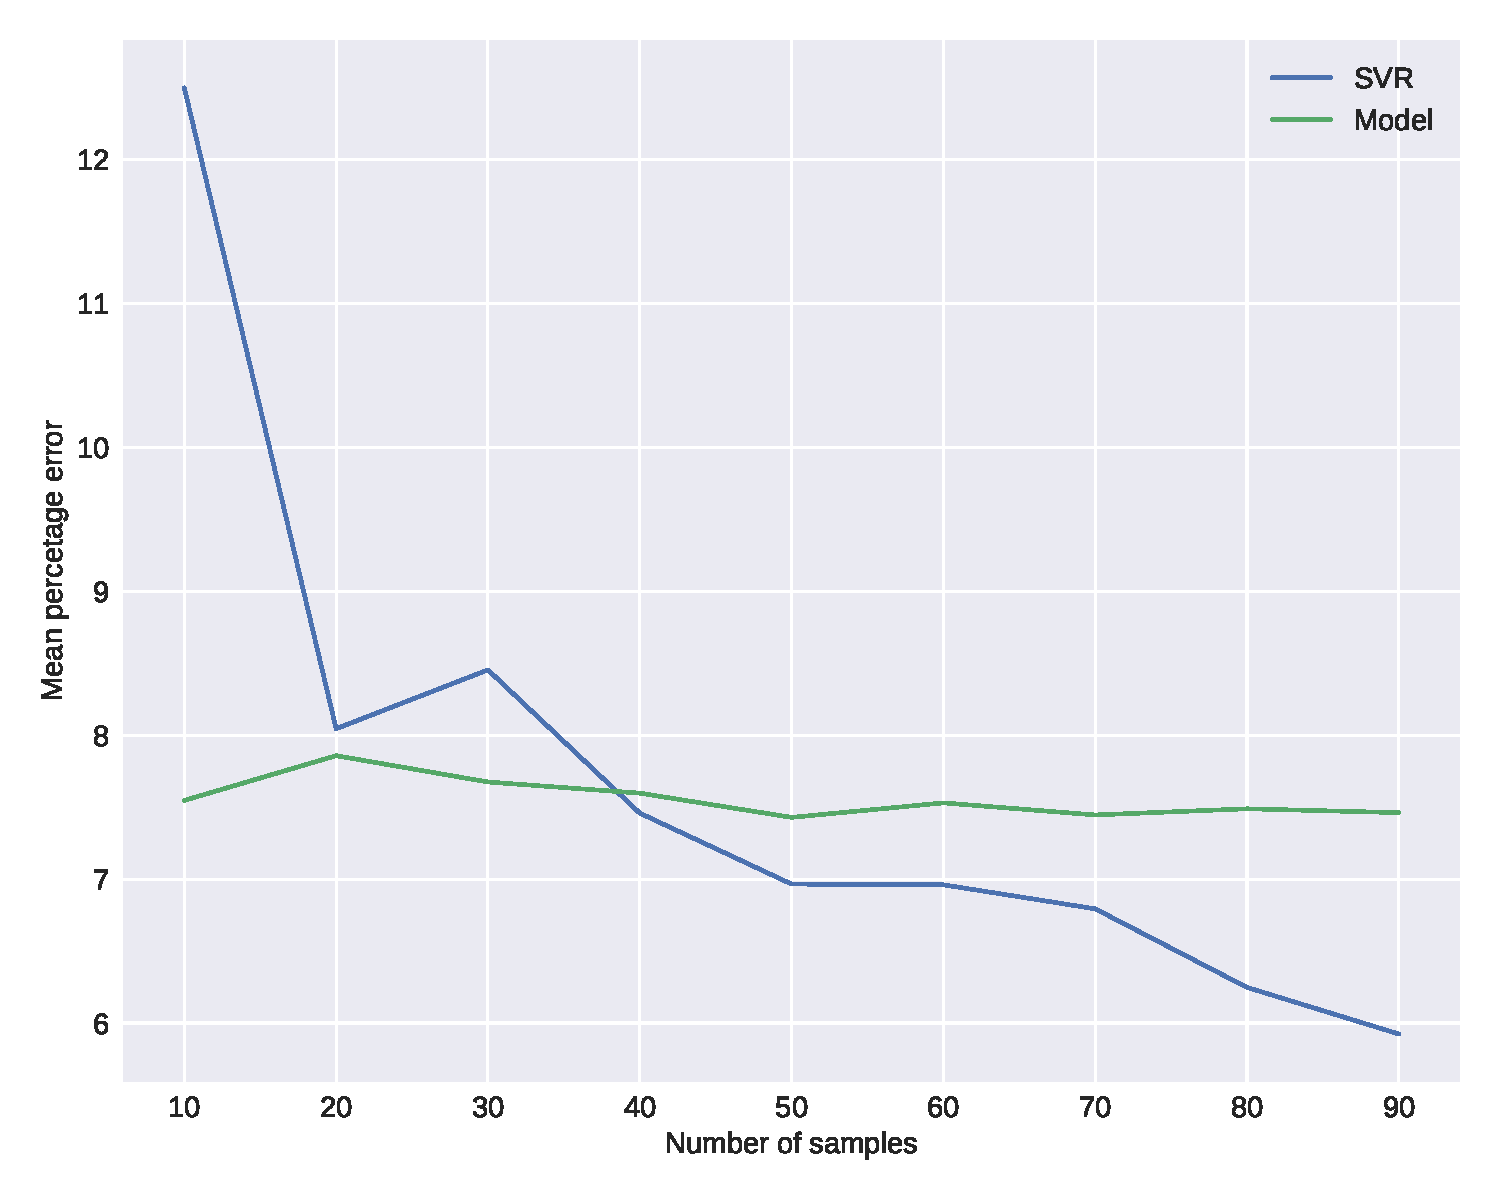
\includegraphics[width=\columnwidth]{models/figures/overhead/completo_ferret_4.png}}
		\caption{MPE for Ferret.}
		\label{fig:overhead_ferret}
	\end{subfigure}
	%
	\begin{subfigure}[b]{0.45\textwidth}
		\centerline{\includegraphics[width=\columnwidth]{models/figures/overhead/completo_vips_4.png}}
		\caption{MPE for Vips.}
		\label{fig:overhead_vips}
	\end{subfigure}
	%
	\begin{subfigure}[b]{0.45\textwidth}
		\centerline{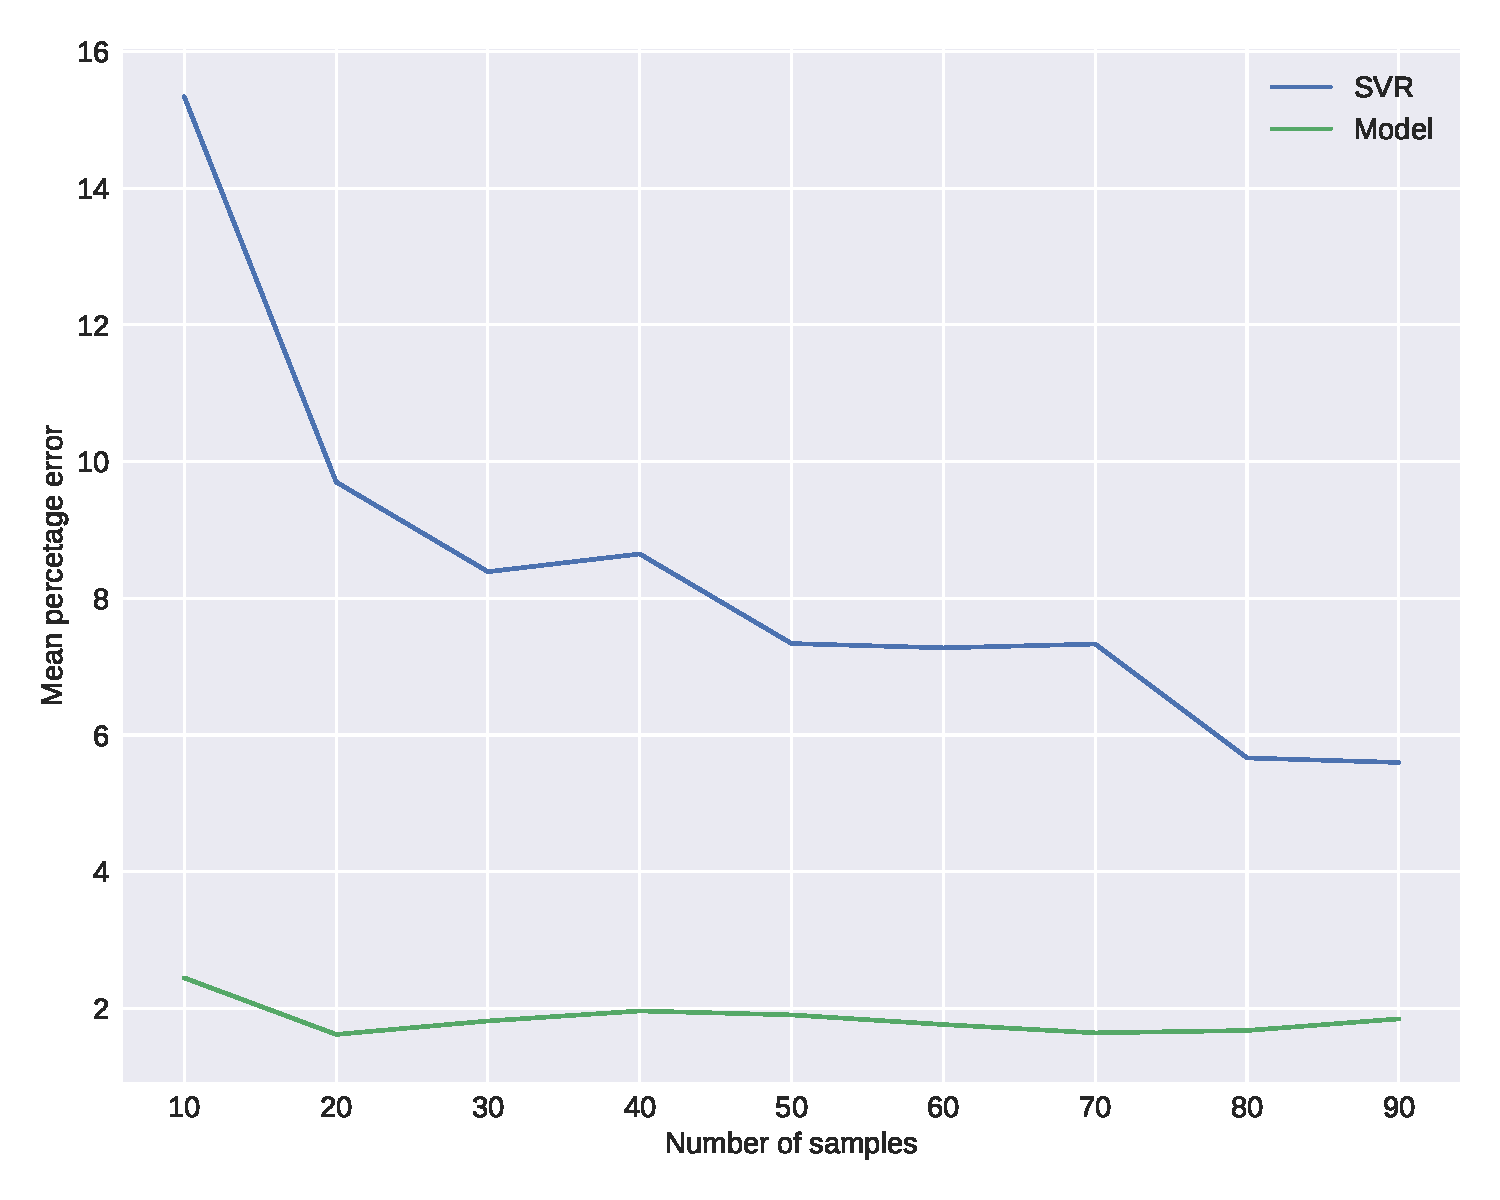
\includegraphics[width=\columnwidth]{models/figures/overhead/completo_x264_4.png}}
		\caption{MPE for x264.}
		\label{fig:overhead_x264}
	\end{subfigure}
	\caption{MPE case studies: Ferret (a), Vips (b) and x264 (c): model (almost constant) versus SVR (lowest MPE beyond train-size 35 on case (b)).}
	\label{fig:overheadFerretVips}
\end{figure}

Figure \ref{fig:overheadFerretVips} shows the comparisons of MPE and energy spent to create each model for two selected applications. According to the results, the analytical model is found to be very stable, not changing much as more data is added, while the SVR keeps reshaping to adapt to the data. 
The error of the analytical model is almost constant but that of  the SVR, initially very high, drops at some point.
\begin{figure}[H]
	\centering
	\begin{subfigure}[b]{0.44\textwidth}
		\centerline{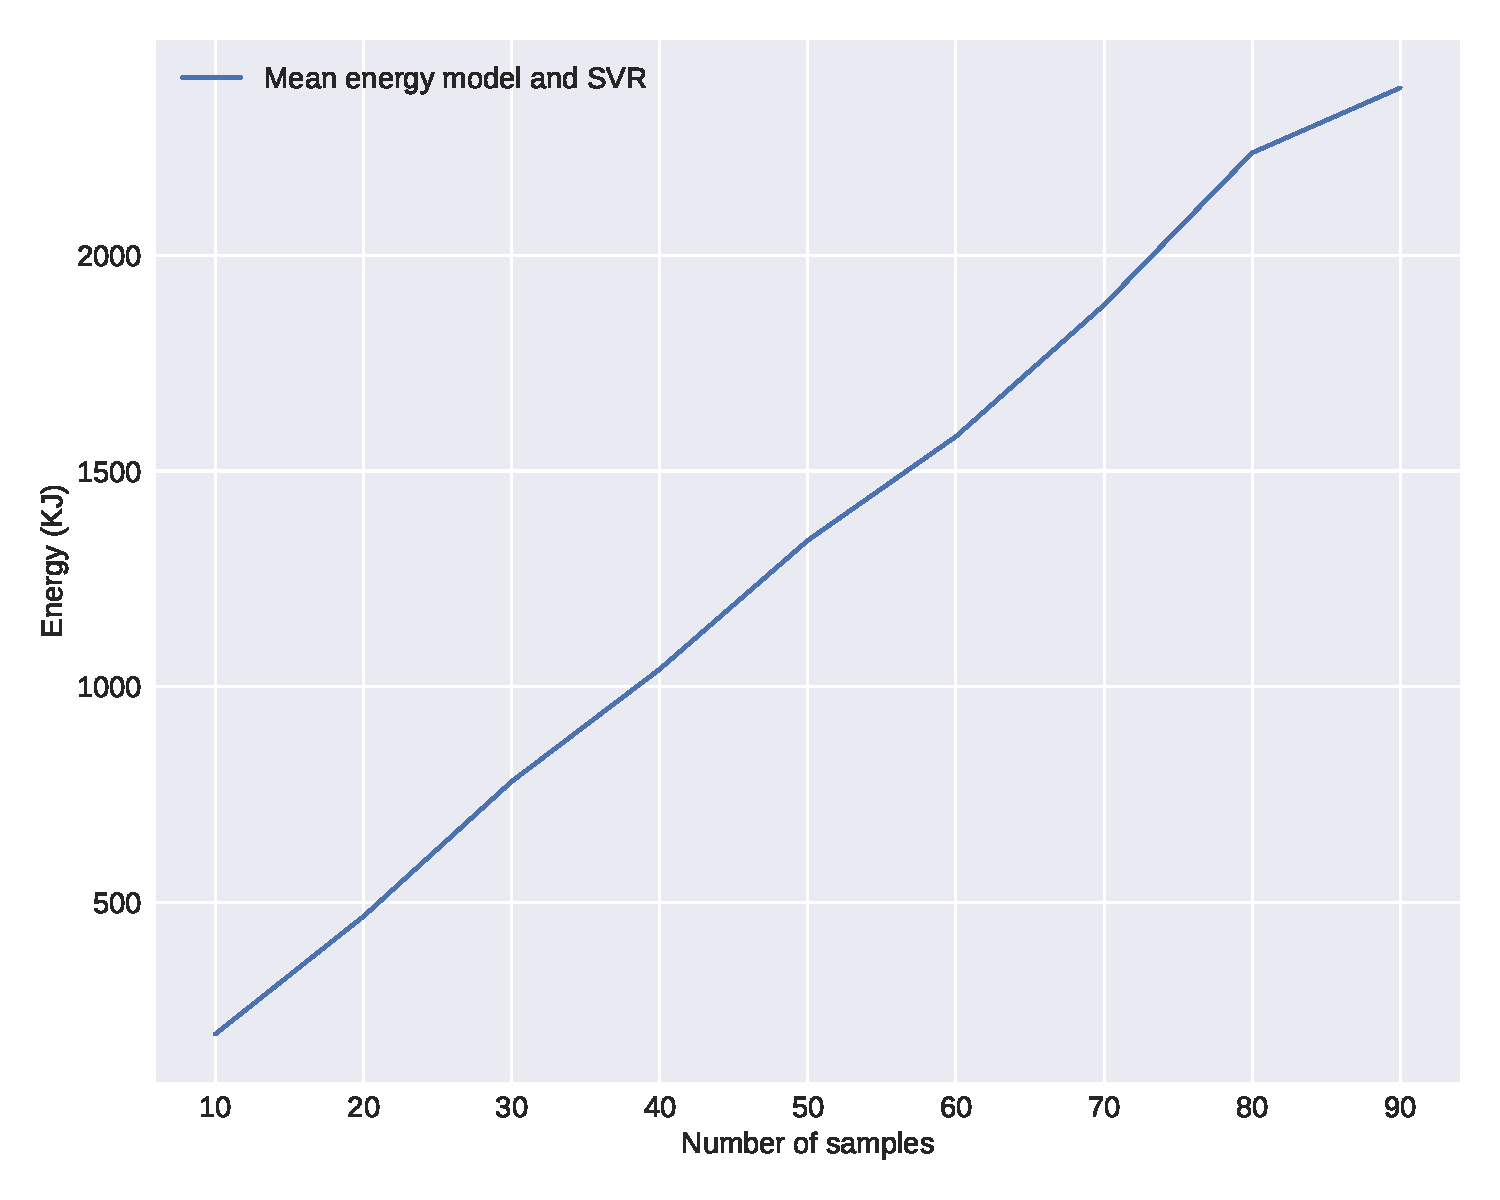
\includegraphics[width=\columnwidth]{models/figures/overhead/overall_energy_10pts.png}}
		\caption{Average energy spent on all applications during model creation. The two curves are identical because the same data were used to adjust the SVR and the model.}
		\label{fig:overall_overhead}
	\end{subfigure}
	%
	\quad
	\begin{subfigure}[b]{0.44\textwidth}
		\centerline{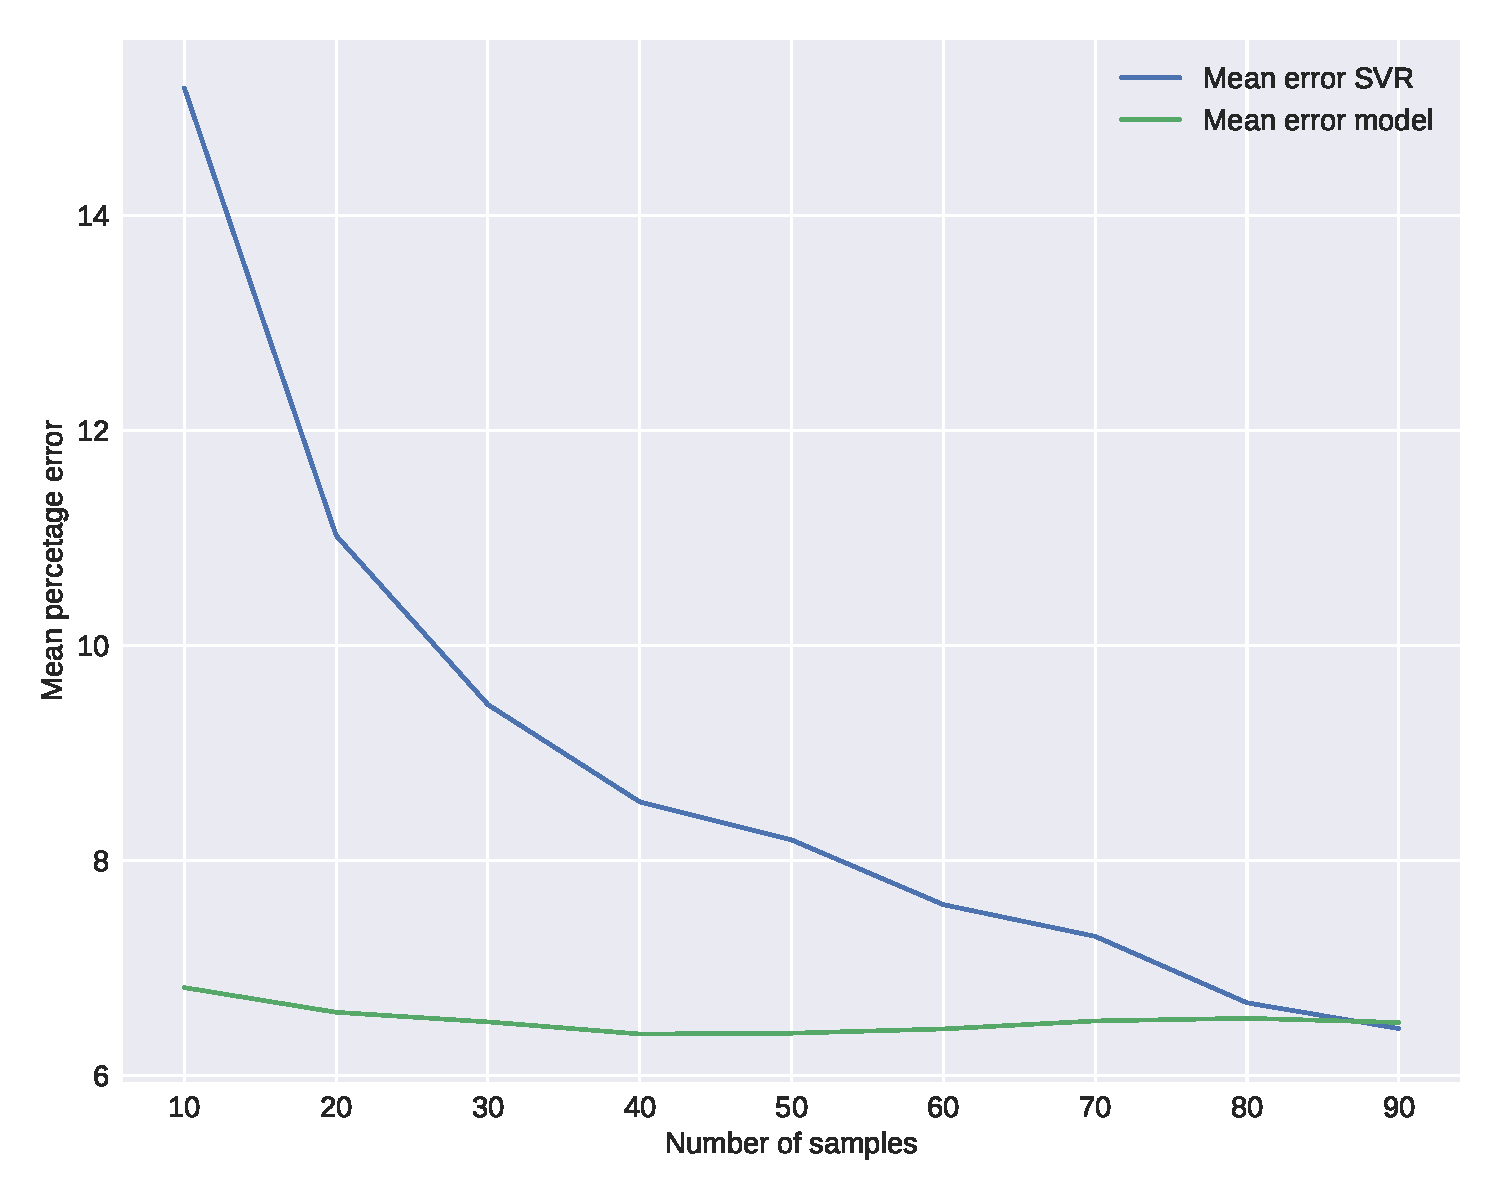
\includegraphics[width=\columnwidth]{models/figures/overhead/overall_mpe_10pts.png}}
		\caption{
			MPE all applications: SVR needs 10 times more data to have an MPE lower than the model.}
		\label{fig:overall_MPE}
	\end{subfigure}
	\caption{Overall results for energy and MPE for each training size.}
	\label{fig:overall_train}
\end{figure}
Figure \ref{fig:overall_train} presents the overall results, with the mean energy overhead and MPE for all applications.
The meeting point of the MPE for the SVR and the proposed model can be extracted from  \ref{fig:overall_MPE}.
There it shows that around 90 configurations the SVR starts to have a smaller error. The cost of that is the linear increase in energy spent on training. The increase in energy, about 10 times more, can be observed in Figure \ref{fig:overall_overhead}.


\section{PMCs}


\section{Energy per instruction}

\begin{lstlisting}
xor rcx, rcx
mov rax, 1
mov rdx, 0

loop:
	targ_inst(*arg)
	targ_inst(*arg)
	targ_inst(*arg)
	targ_inst(*arg)
	targ_inst(*arg)
	targ_inst(*arg)
	targ_inst(*arg)
	targ_inst(*arg)
	targ_inst(*arg)

add rcx, 1
cmp rcx, 9999999
jne loop
\end{lstlisting}

Estimating the energy of the instruction from this benchmark

$E_{total}=9999999(\frac{10}{13}inst+\frac{3}{13}loop)$

$E_{total}=7692306*inst+constant$

\subsection{Generic}

\begin{figure}
	\centering
	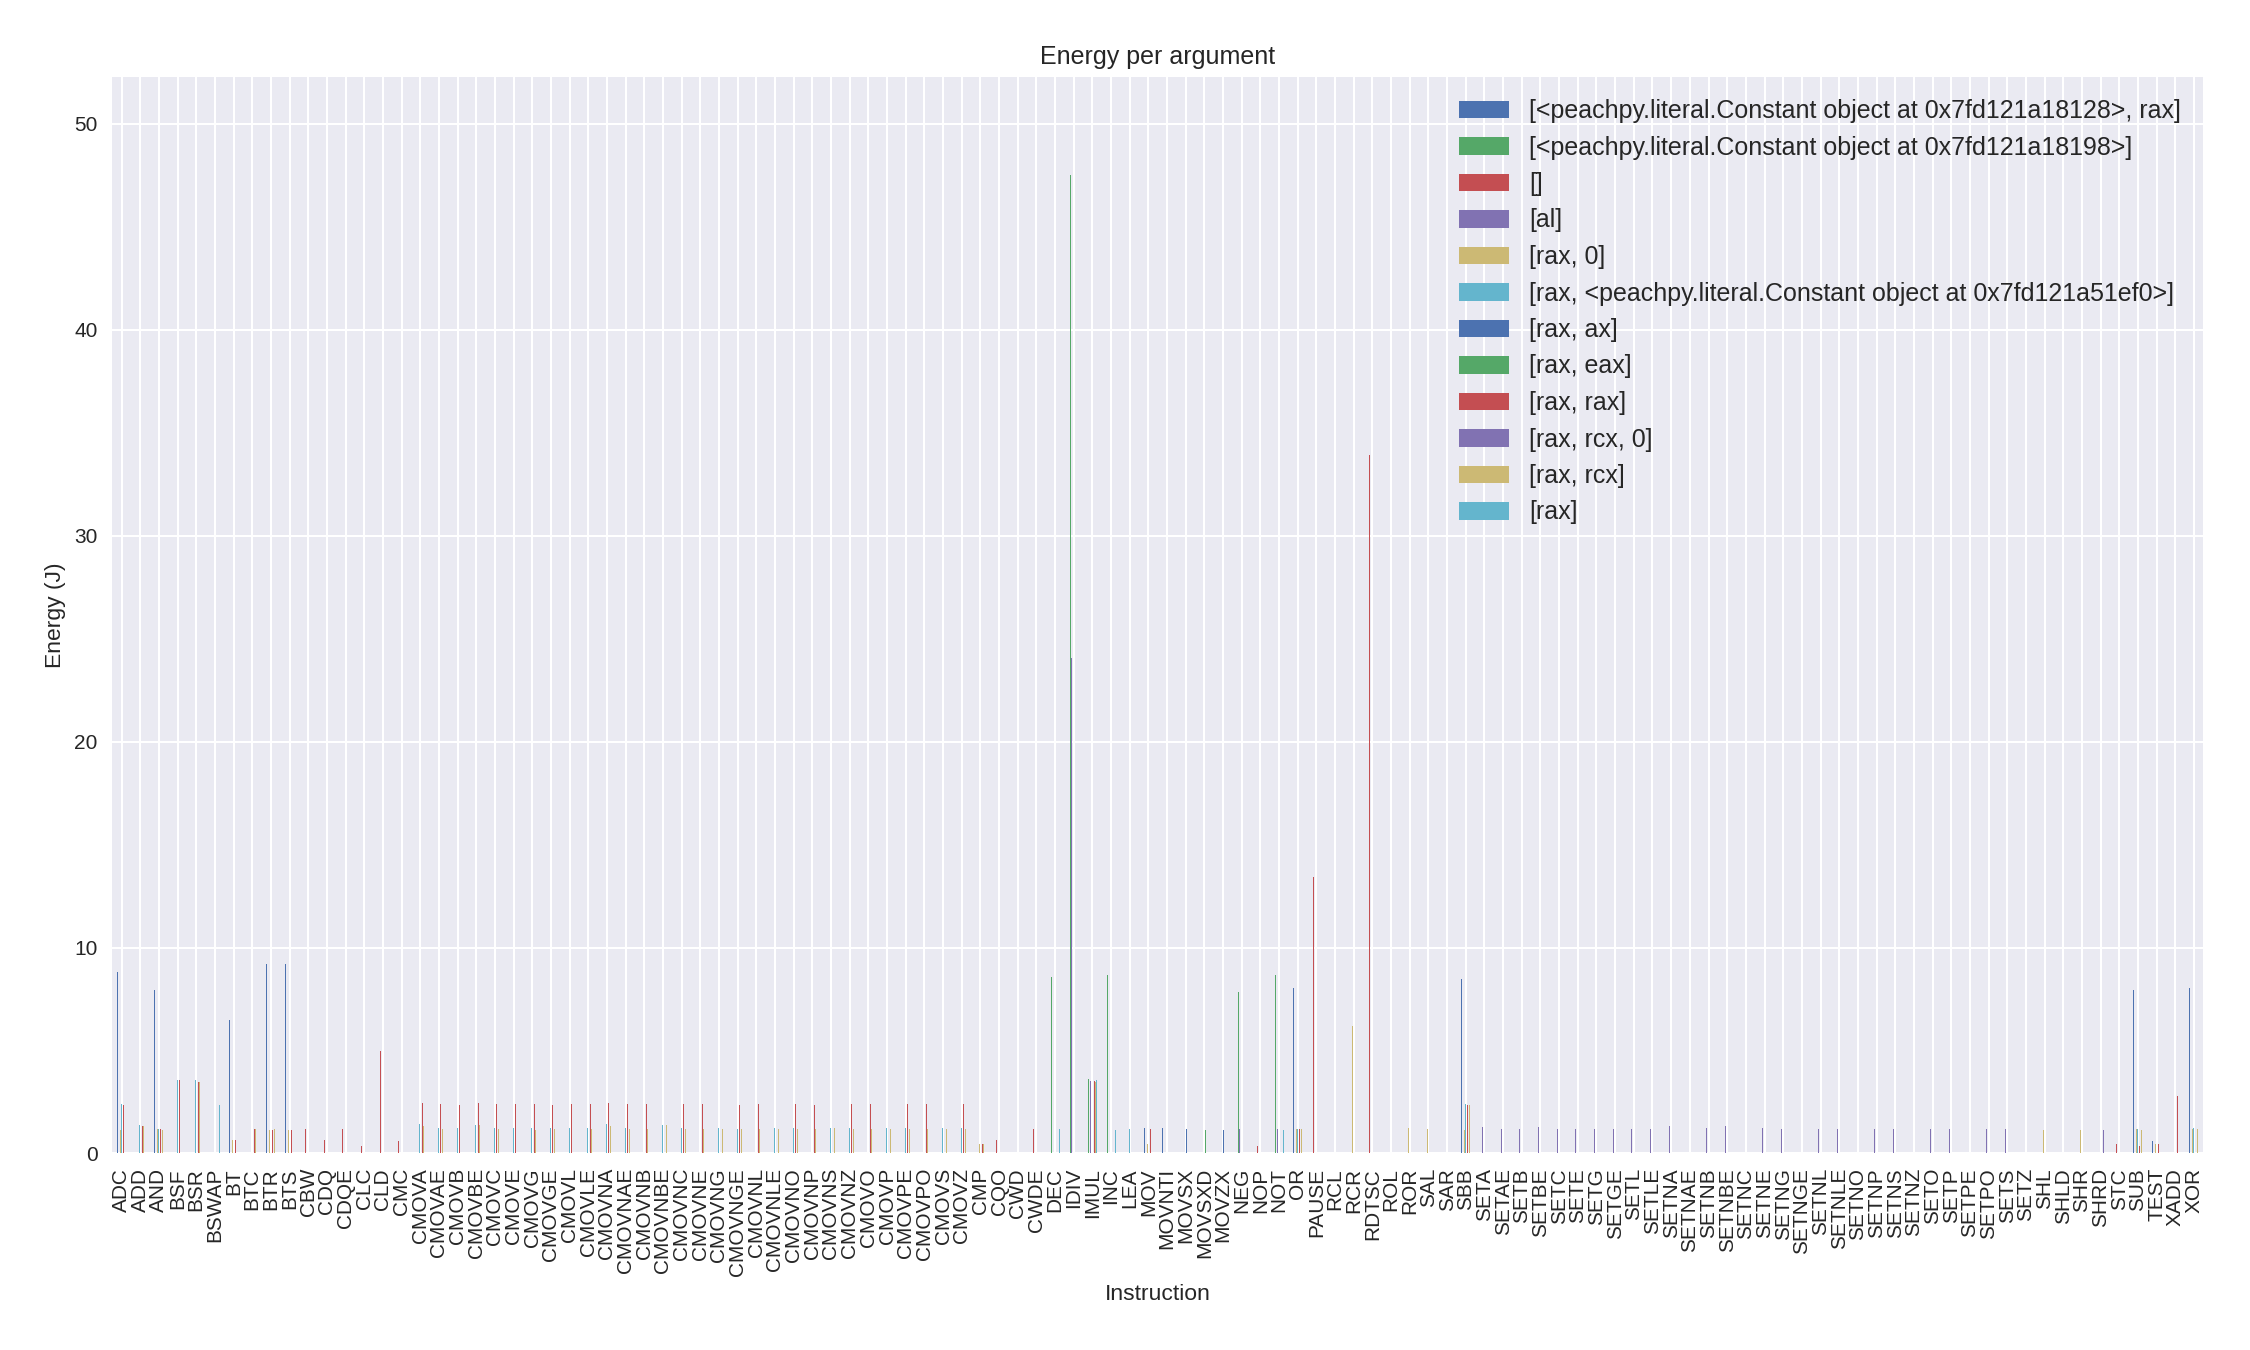
\includegraphics[width=\textwidth]{experiments/figures/inst_en_args_generic.png}
	\caption{Energy per instruction argument}
	\label{fig:experiment_en1}
\end{figure}

\begin{figure}
	\centering
	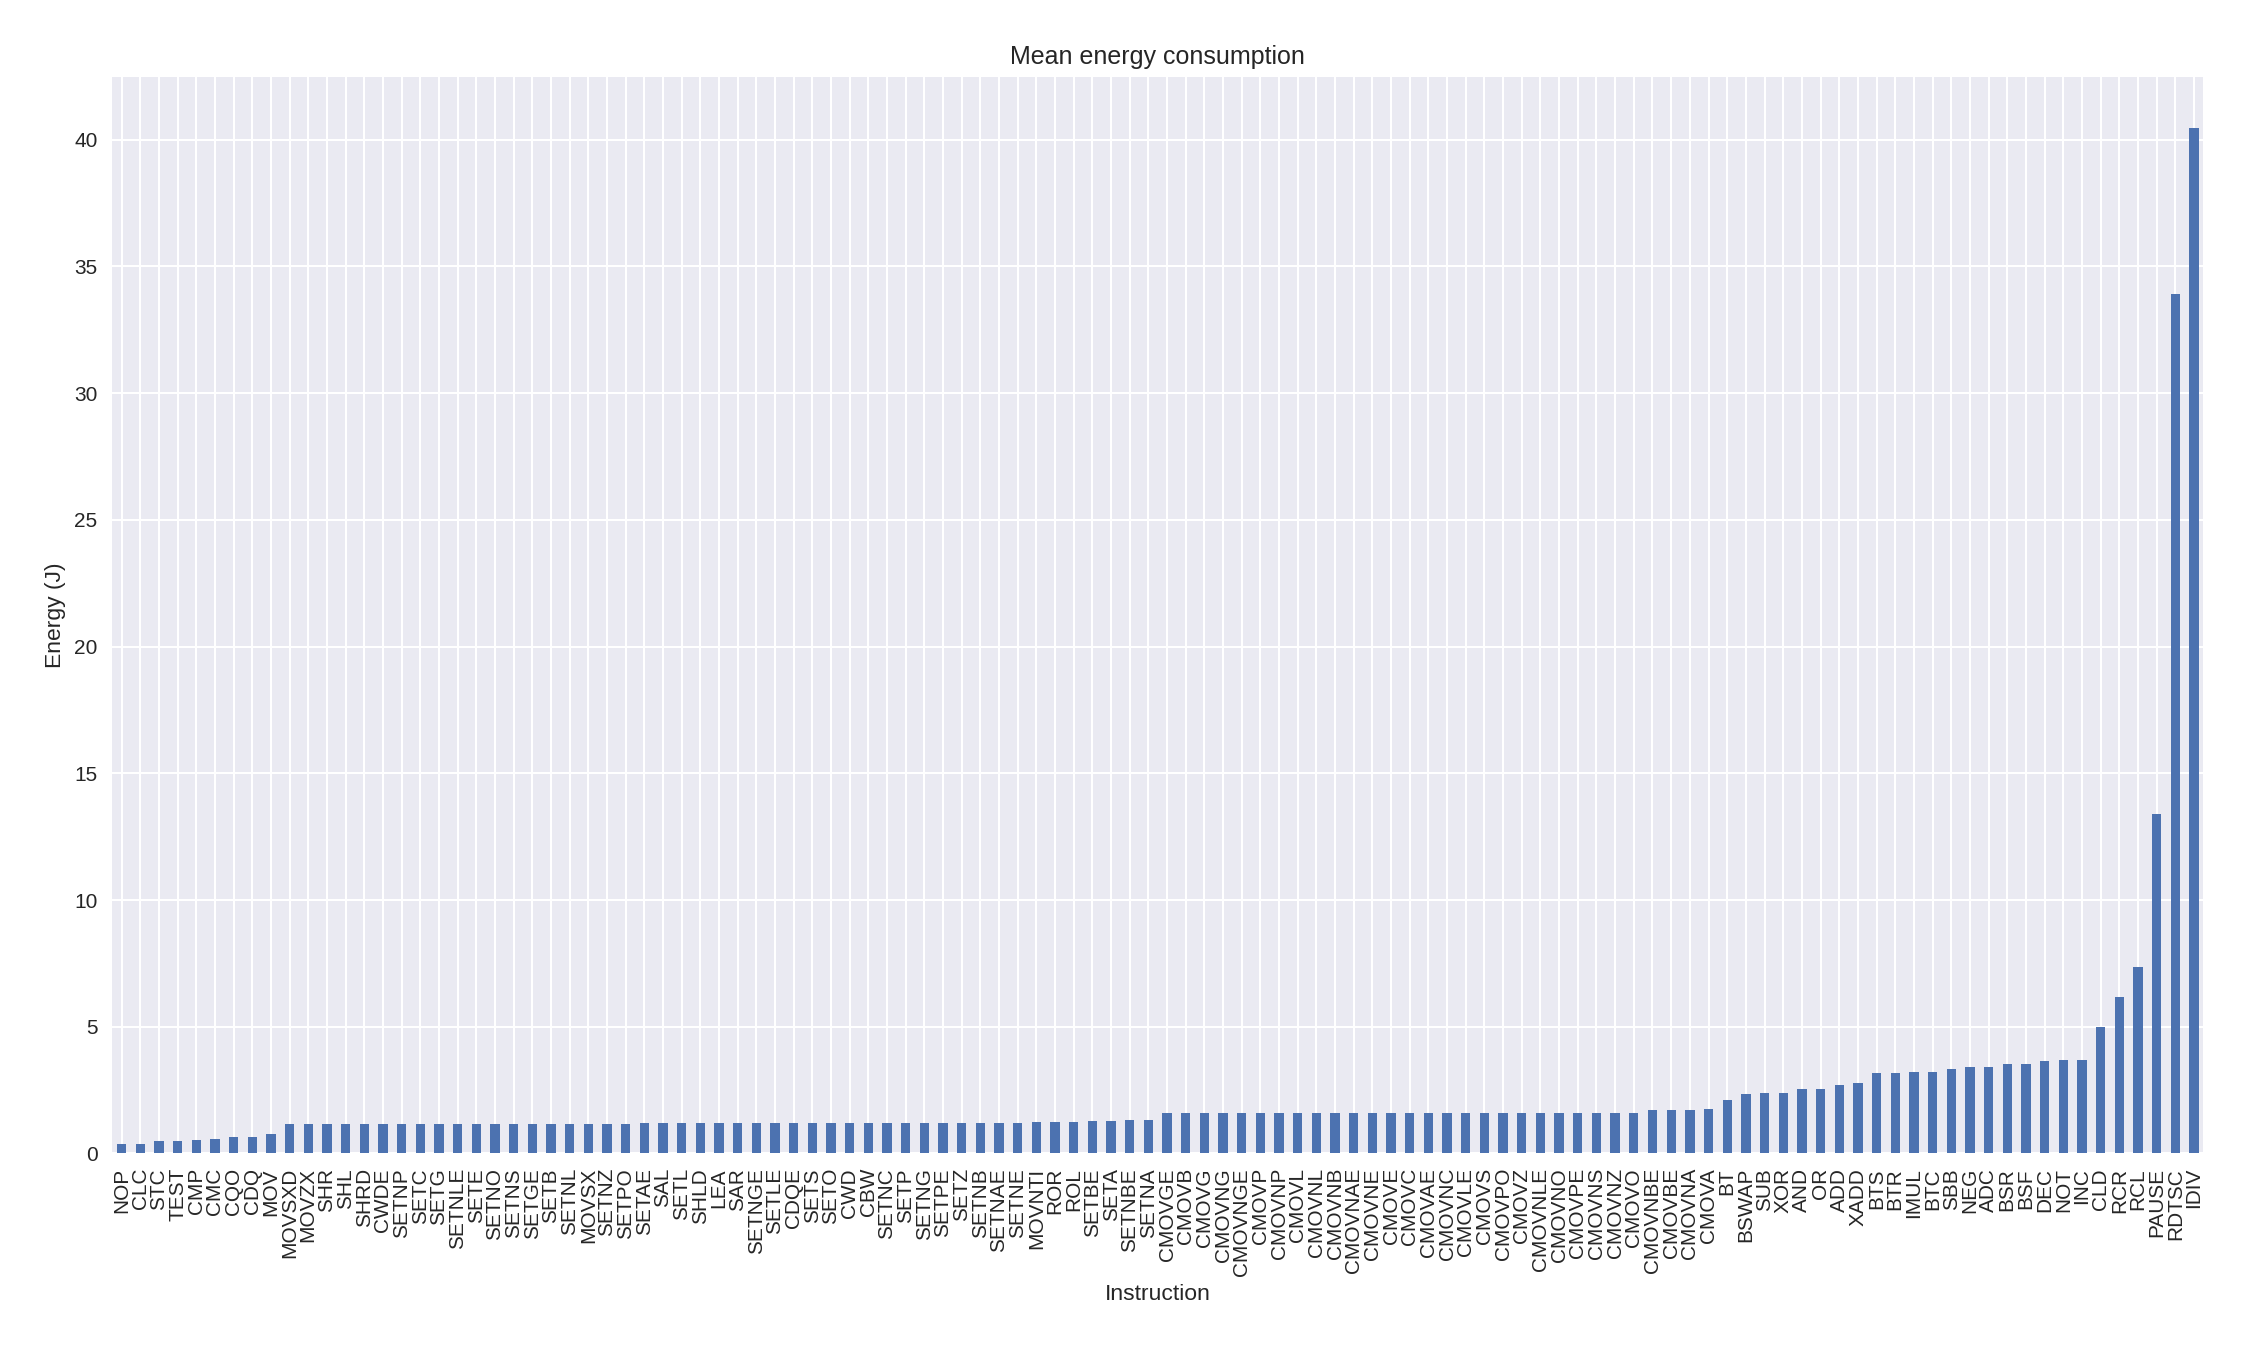
\includegraphics[width=\textwidth]{experiments/figures/inst_mean_en_generic.png}
	\caption{Mean energy per instruction over all arguments}
	\label{fig:experiment_en2}
\end{figure}

\begin{figure}
	\centering
	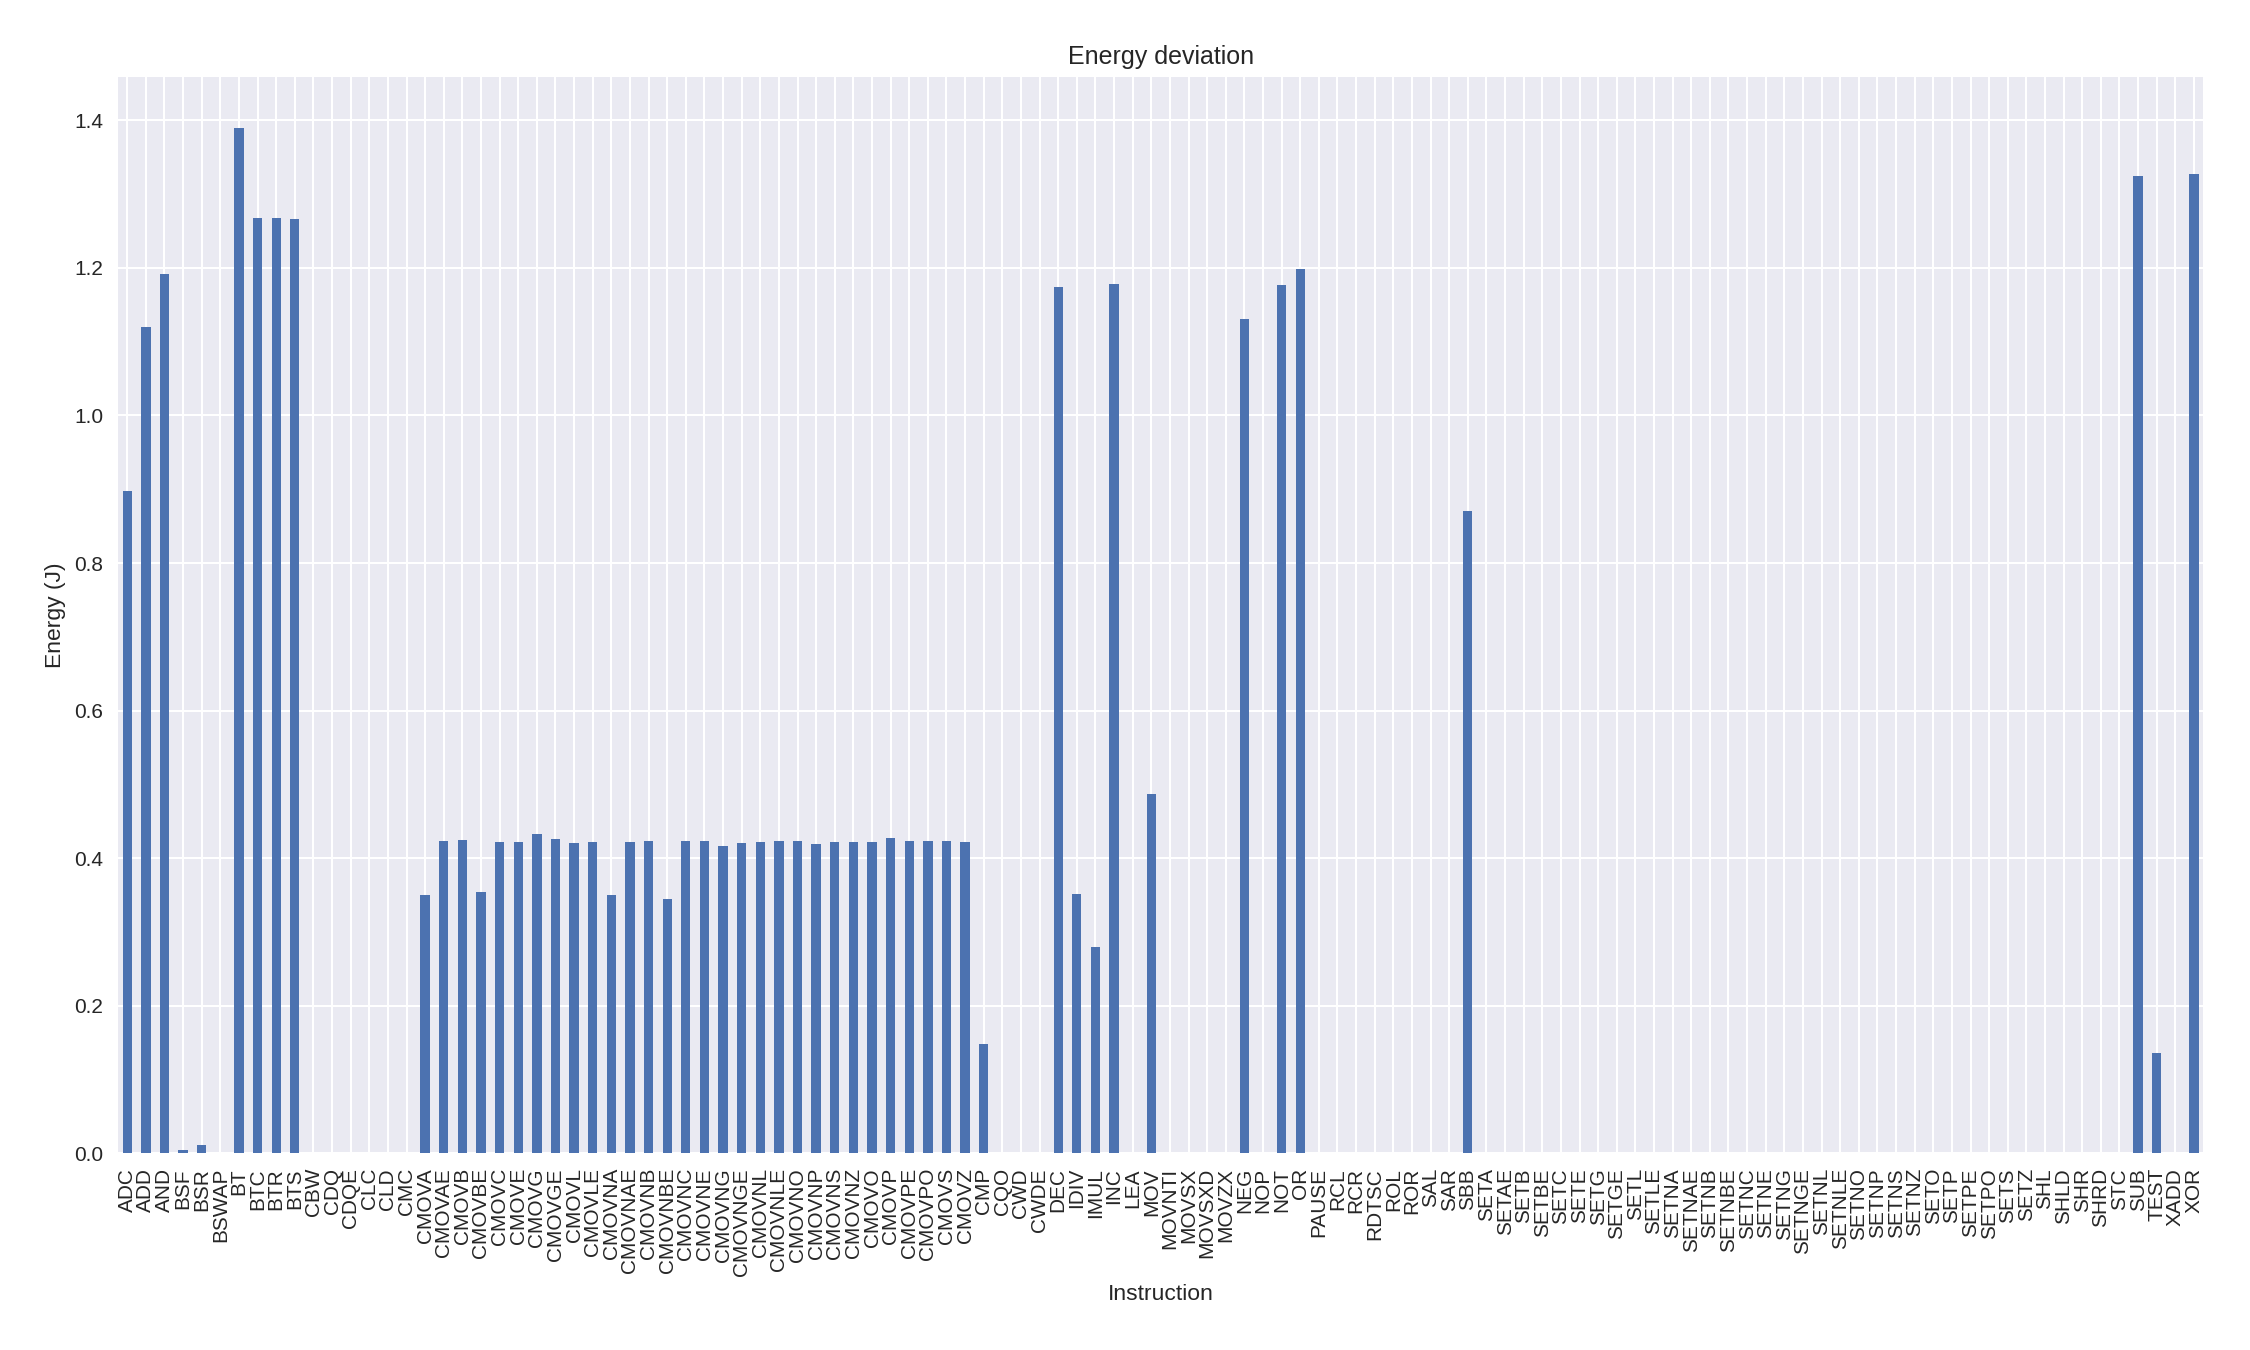
\includegraphics[width=\textwidth]{experiments/figures/inst_std_en_generic.png}
	\caption{Standard deviation energy per instruction over all arguments}
	\label{fig:experiment_en3}
\end{figure}

\subsection{SSE}

\begin{figure}
	\centering
	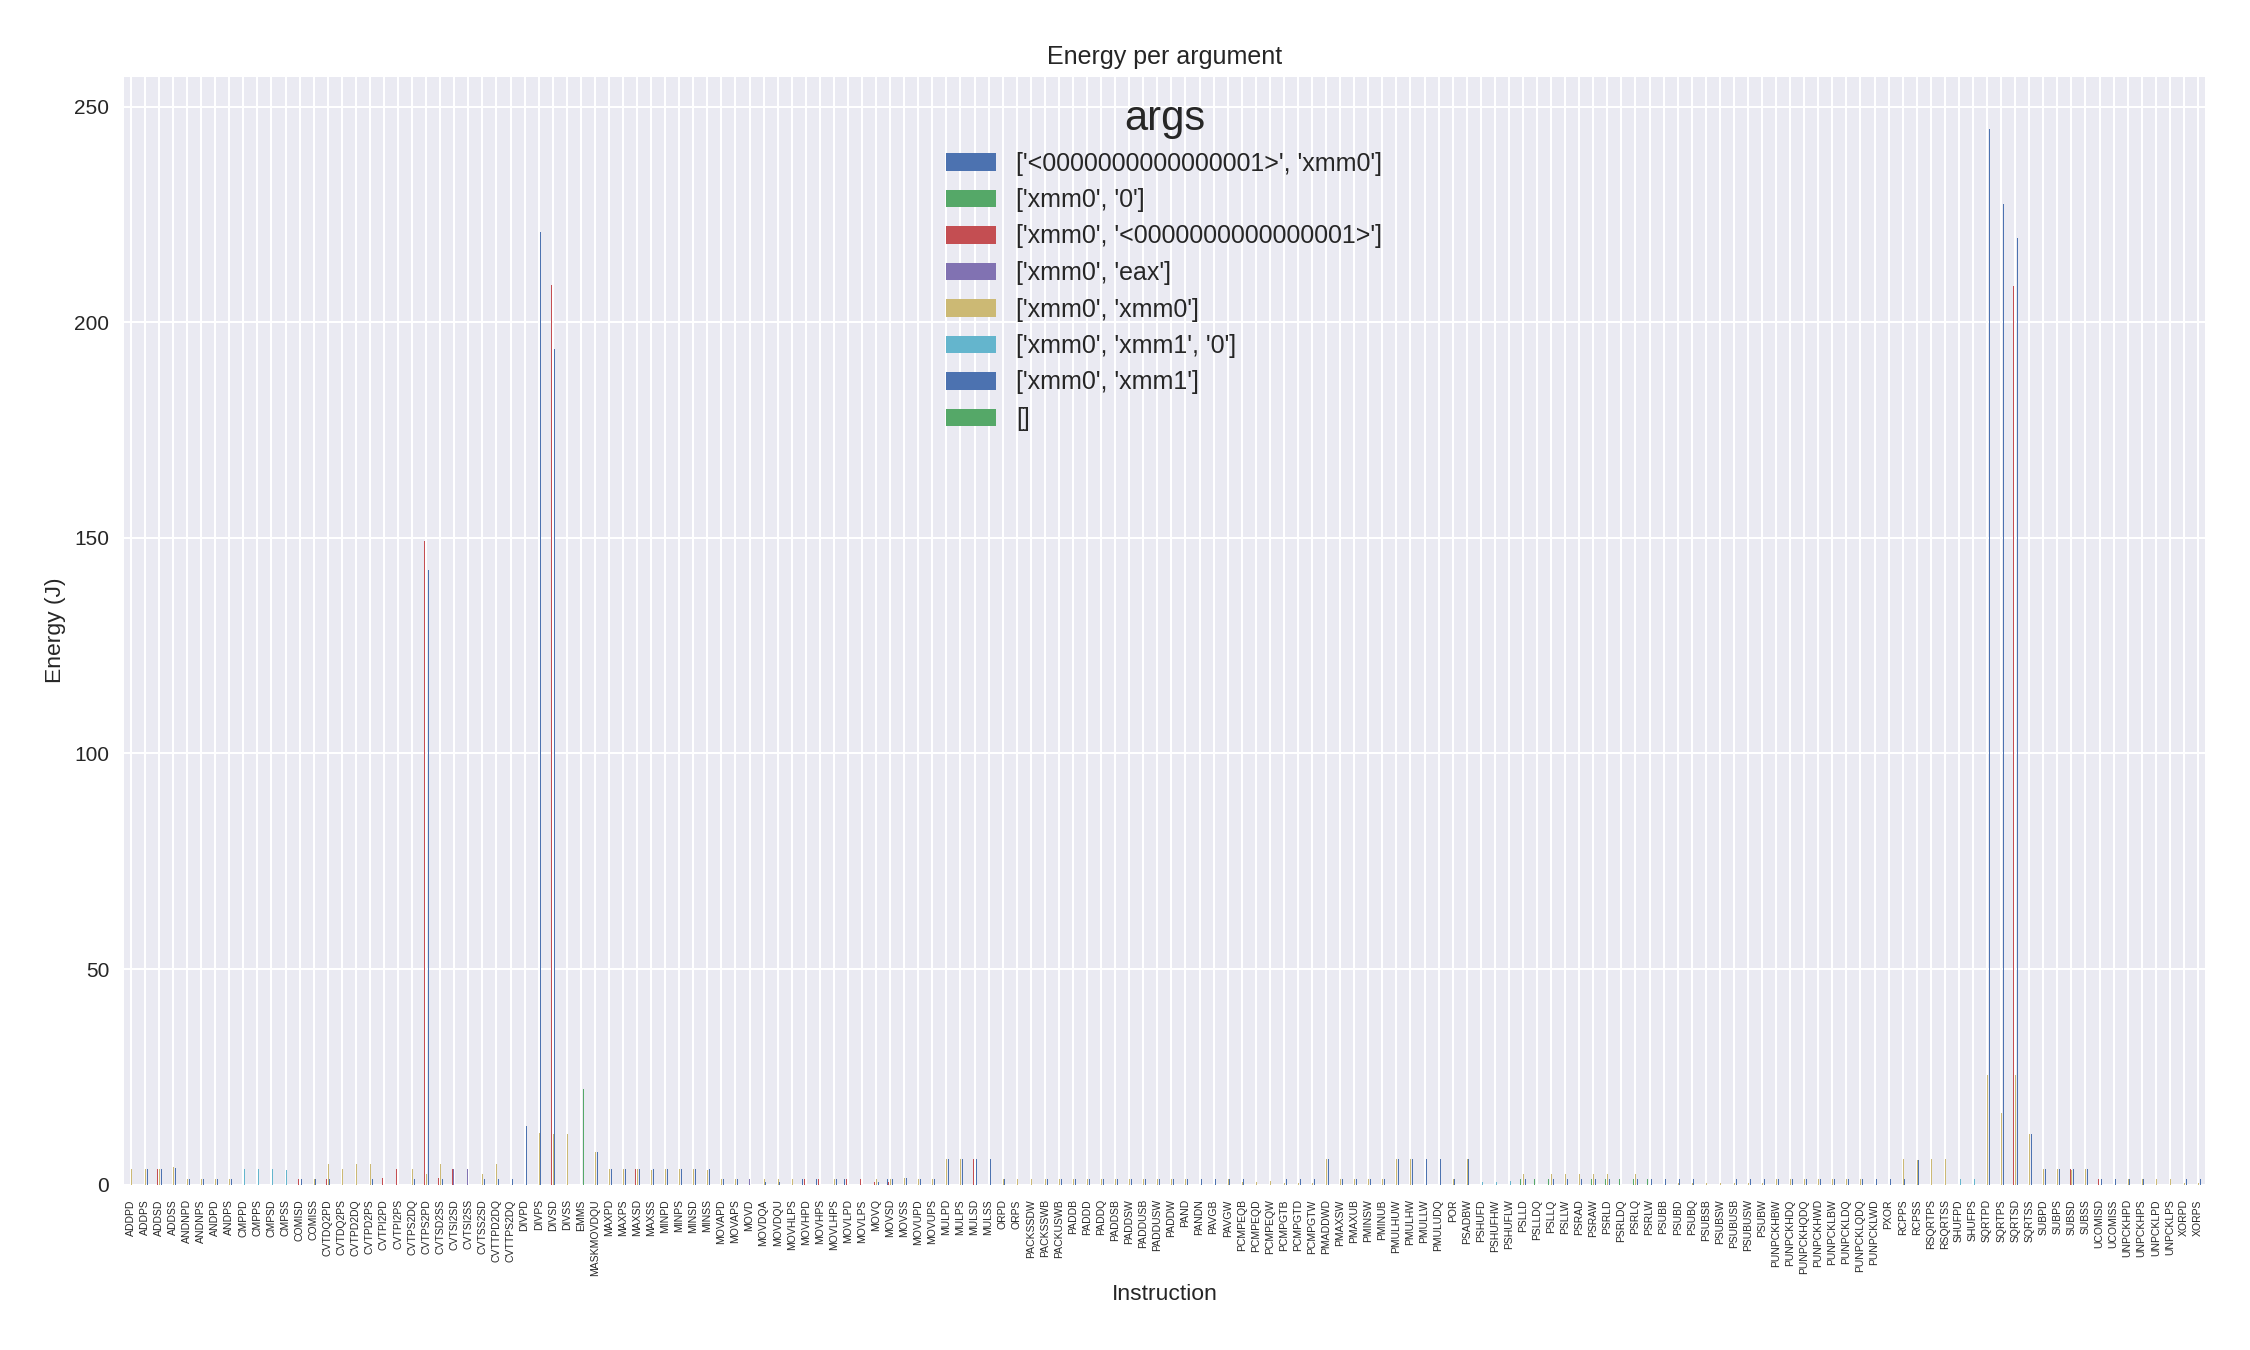
\includegraphics[width=\textwidth]{experiments/figures/inst_en_args_sse.png}
	\caption{Energy per instruction argument (sse)}
	\label{fig:experiment_en4}
\end{figure}

\begin{figure}
	\centering
	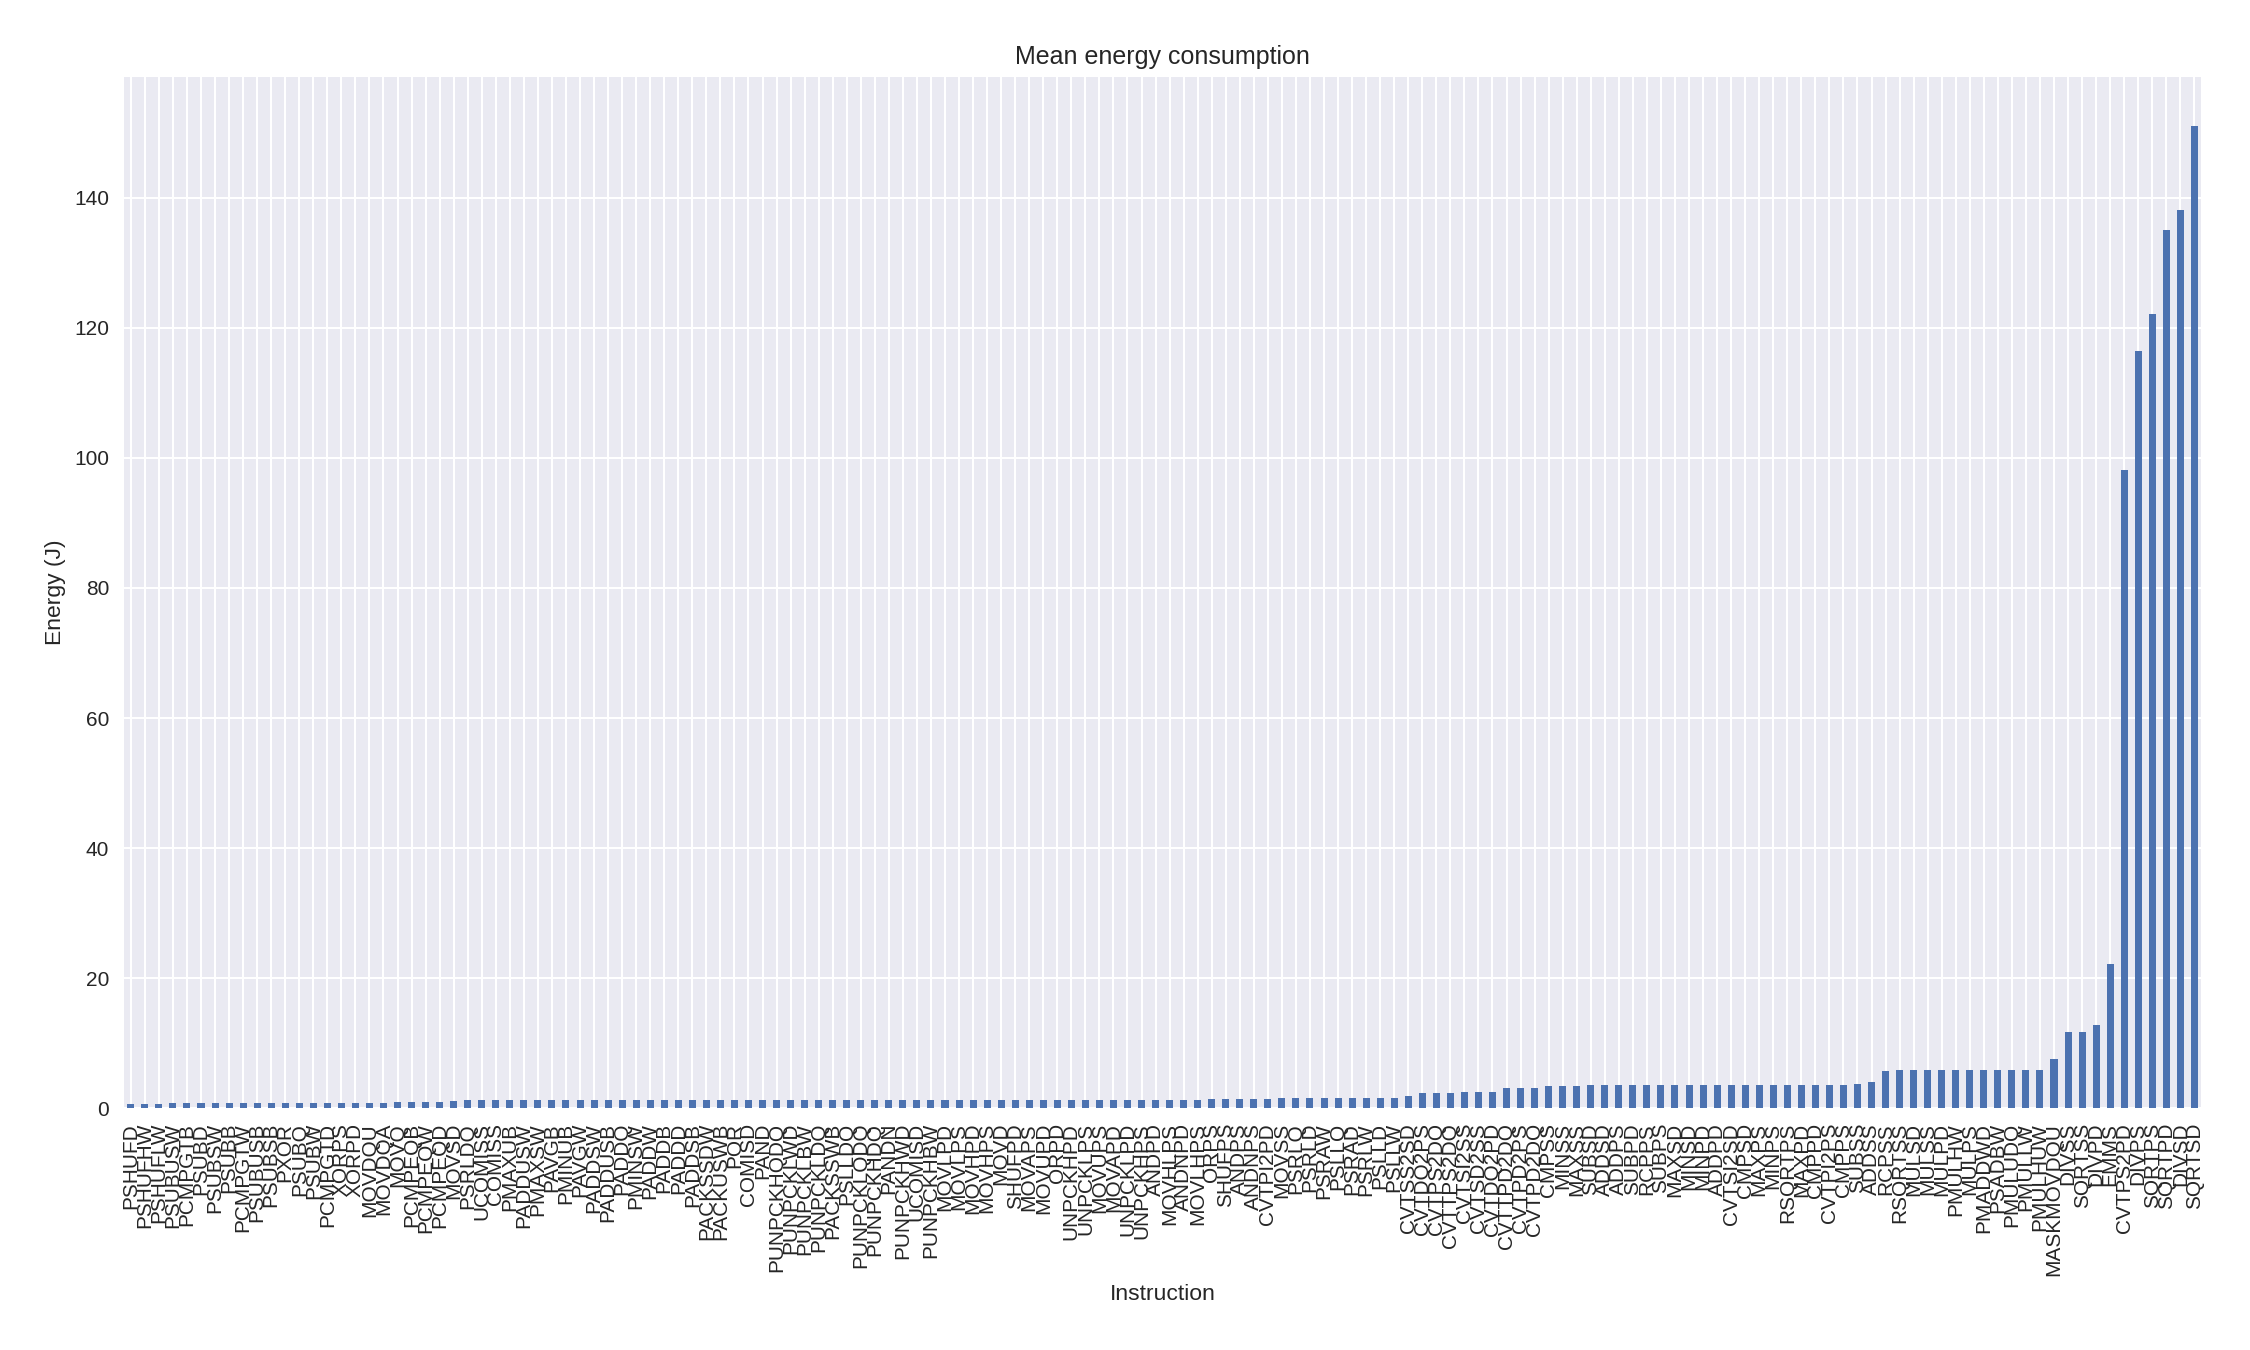
\includegraphics[width=\textwidth]{experiments/figures/inst_mean_en_sse.png}
	\caption{Mean energy per instruction over all arguments (sse)}
	\label{fig:experiment_en5}
\end{figure}

\begin{figure}
	\centering
	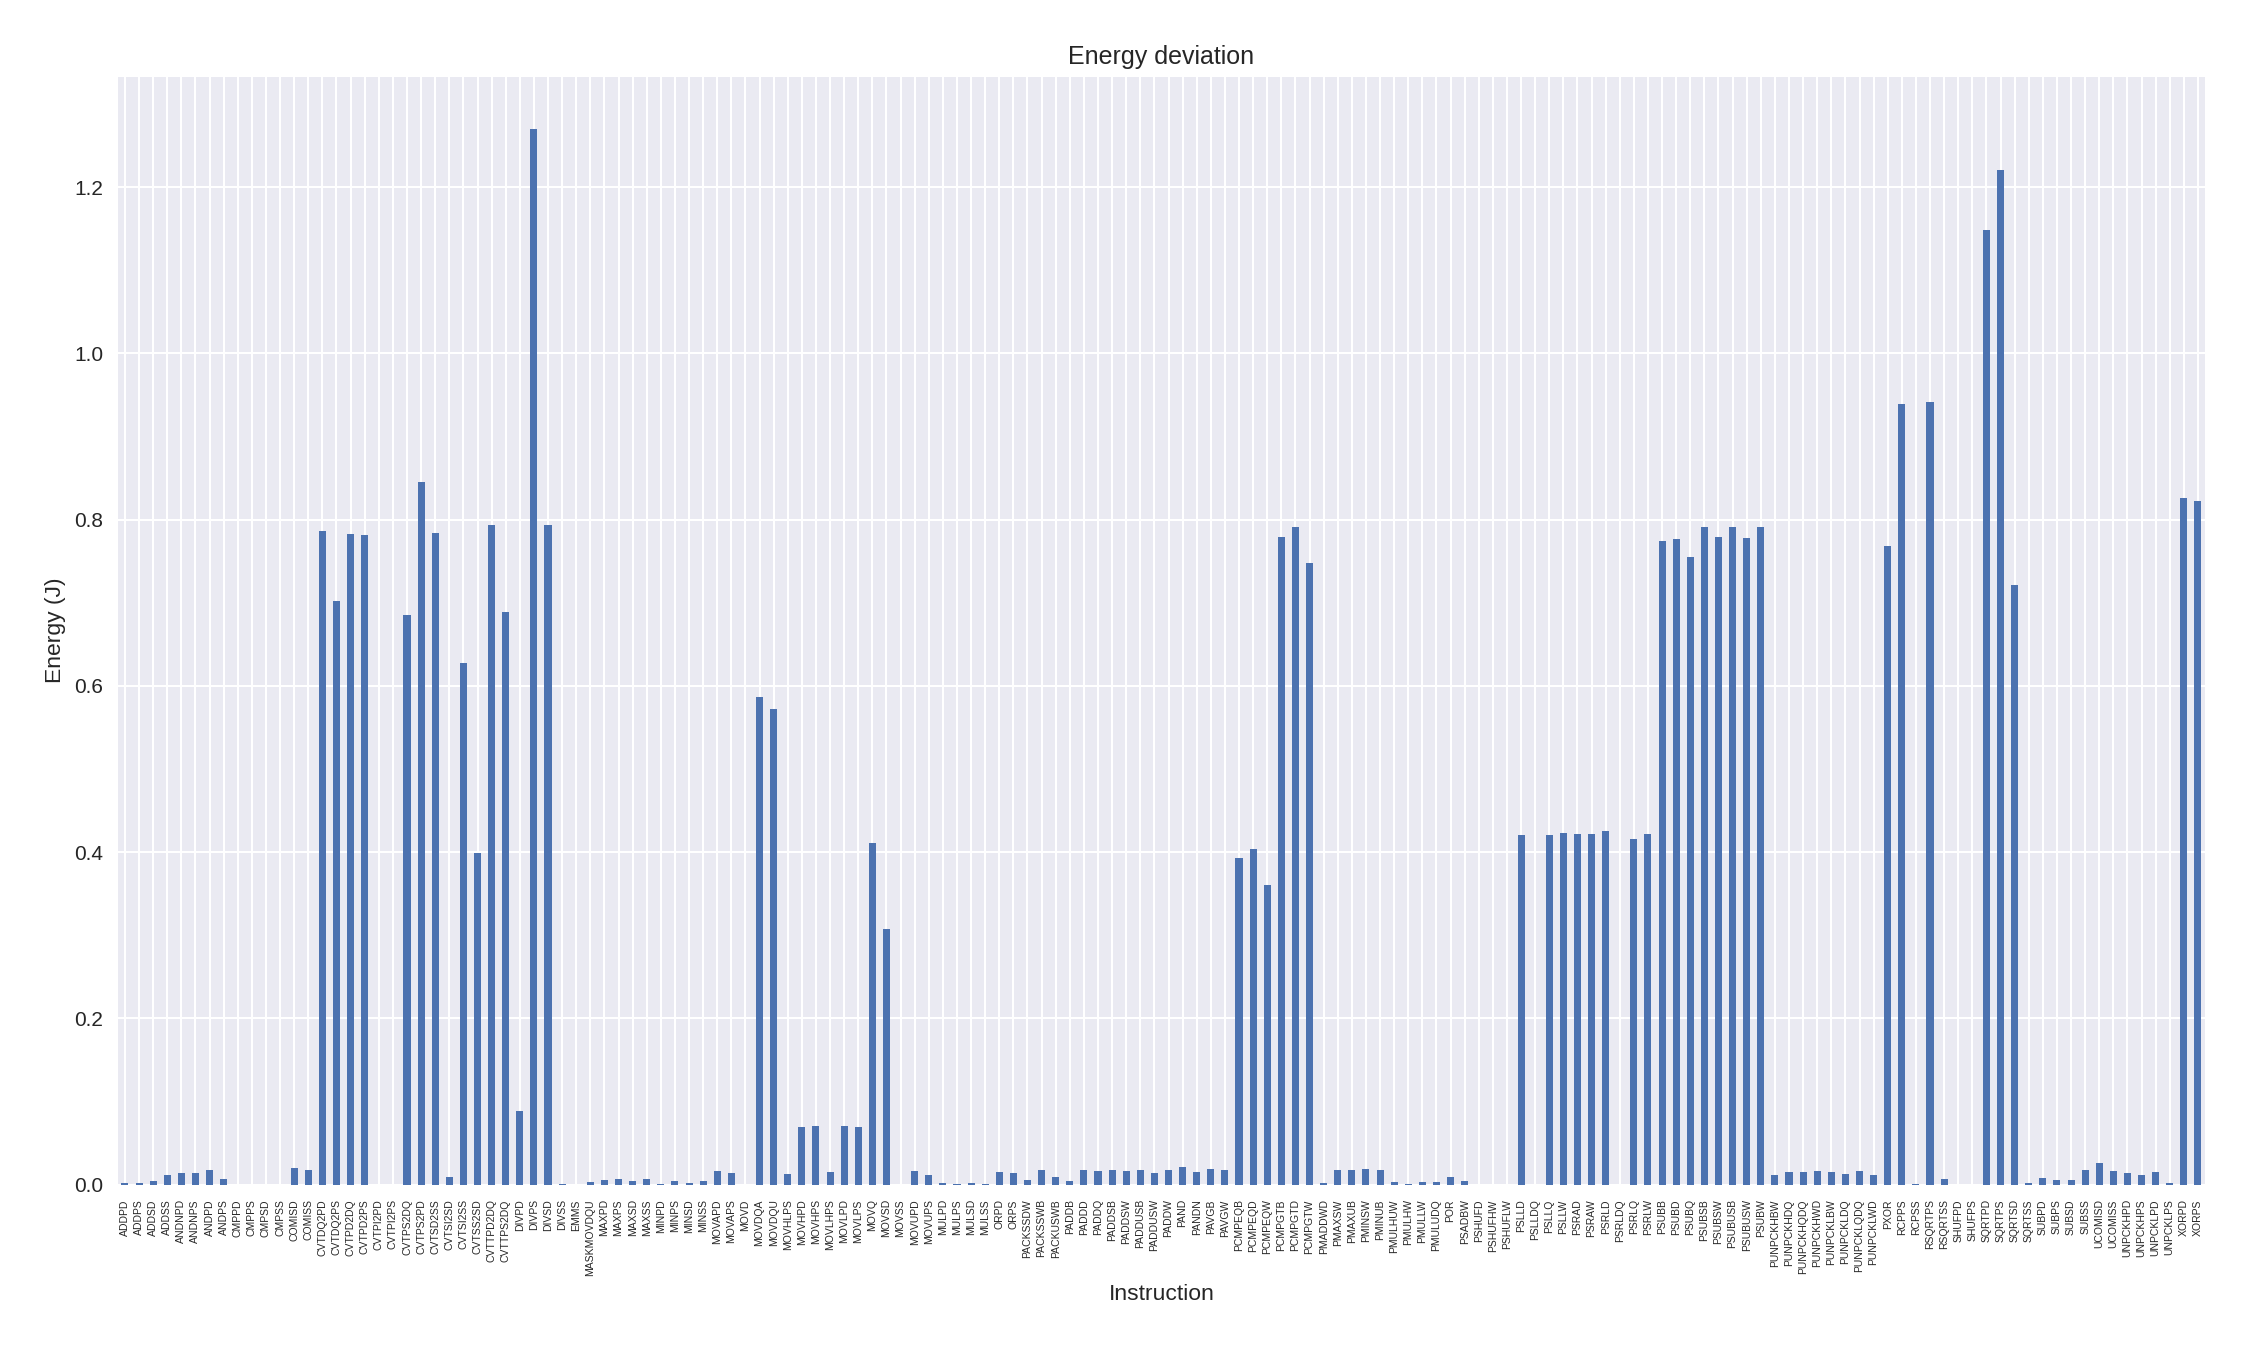
\includegraphics[width=\textwidth]{experiments/figures/inst_std_en_sse.png}
	\caption{Standard deviation energy per instruction over all arguments (sse)}
	\label{fig:experiment_en6}
\end{figure}

\section{SSE and Generic}

\begin{figure}
	\centering
	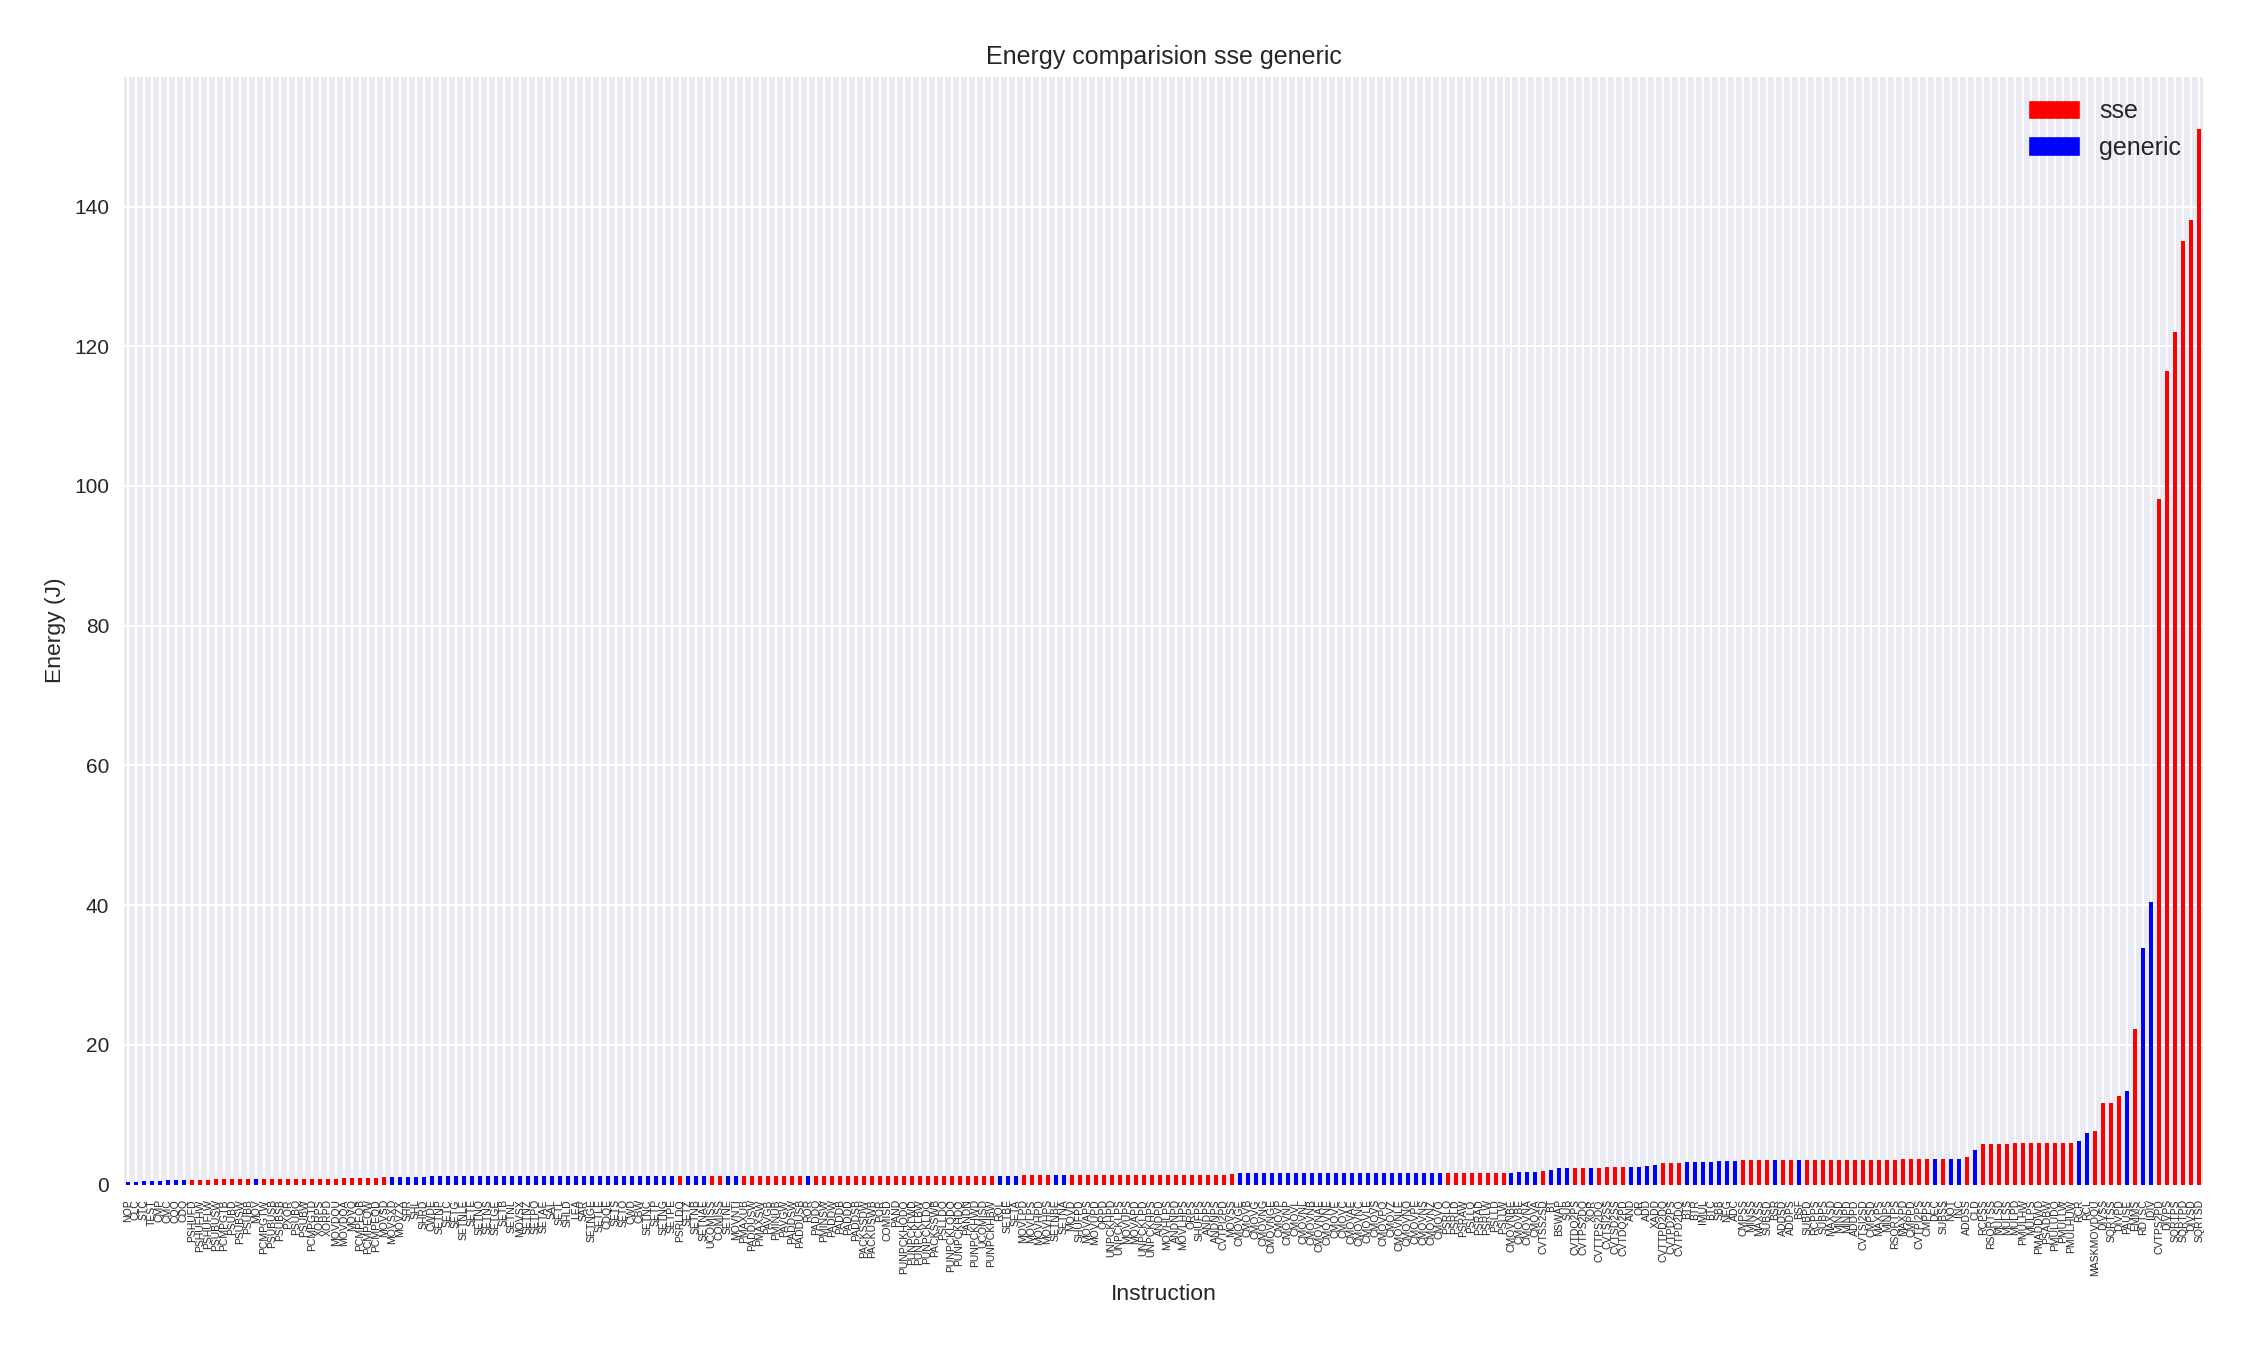
\includegraphics[width=\textwidth]{experiments/figures/inst_en_cmp_sse_generic.png}
	\caption{Comparing SSE and generic instructions energy consumption}
	\label{fig:experiment_en7}
\end{figure}

\section{Power}

\begin{figure}
	\centering
	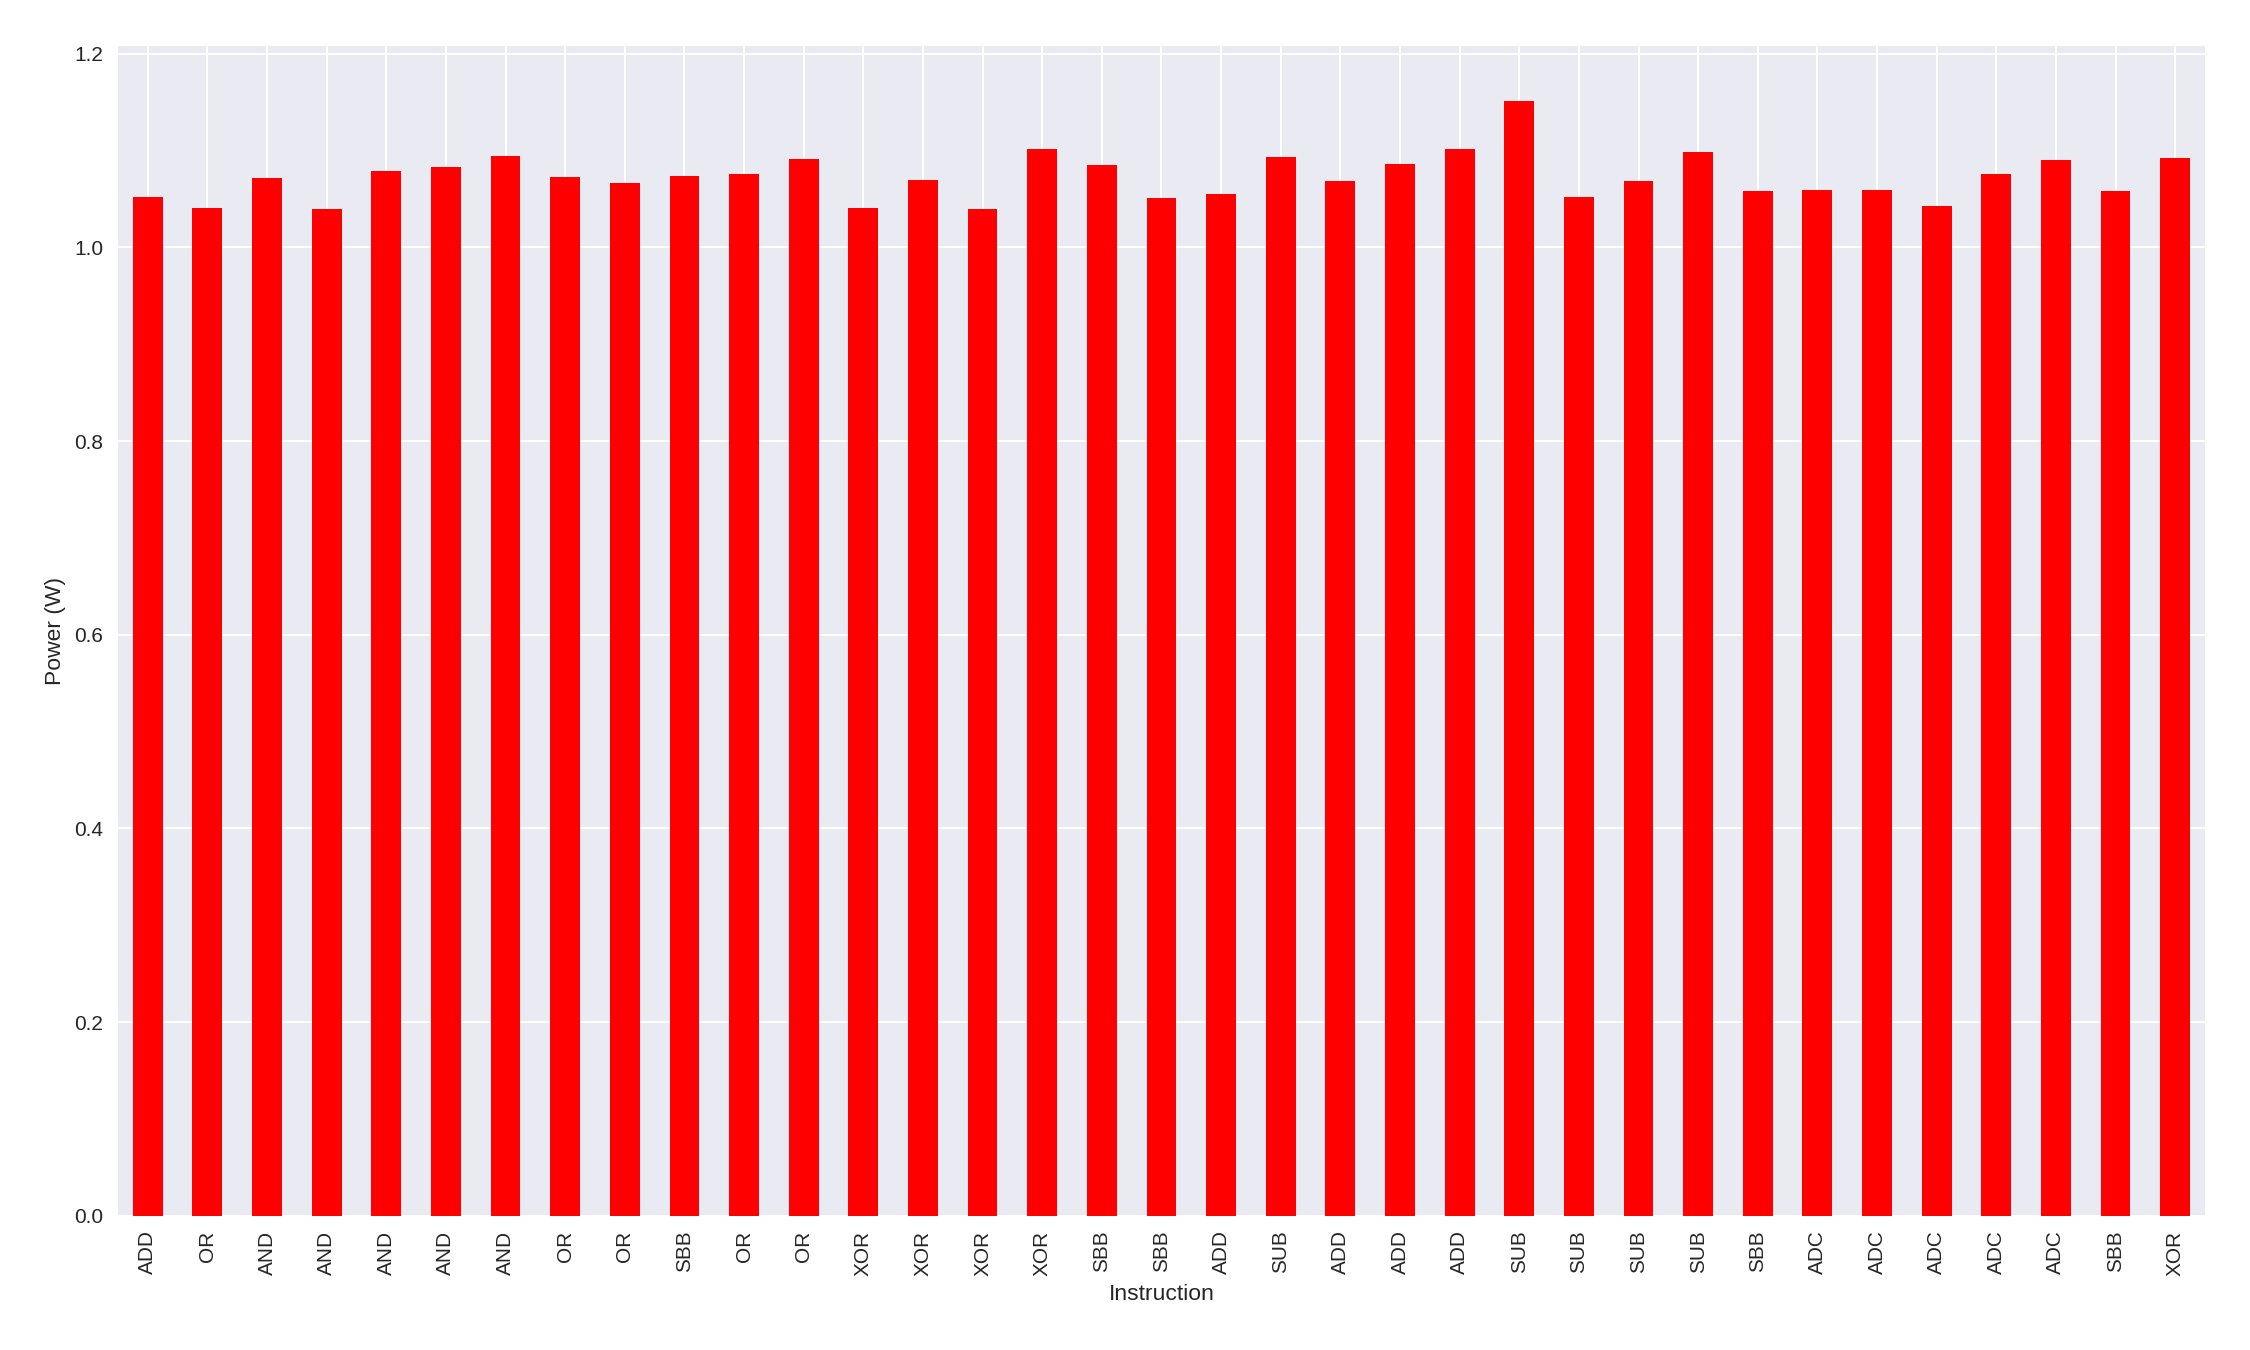
\includegraphics[width=\textwidth]{experiments/figures/inst_pw_generic.png}
	\caption{Instructions power draw}
	\label{fig:experiment_pw1}
\end{figure}
\begin{figure}
	\centering
	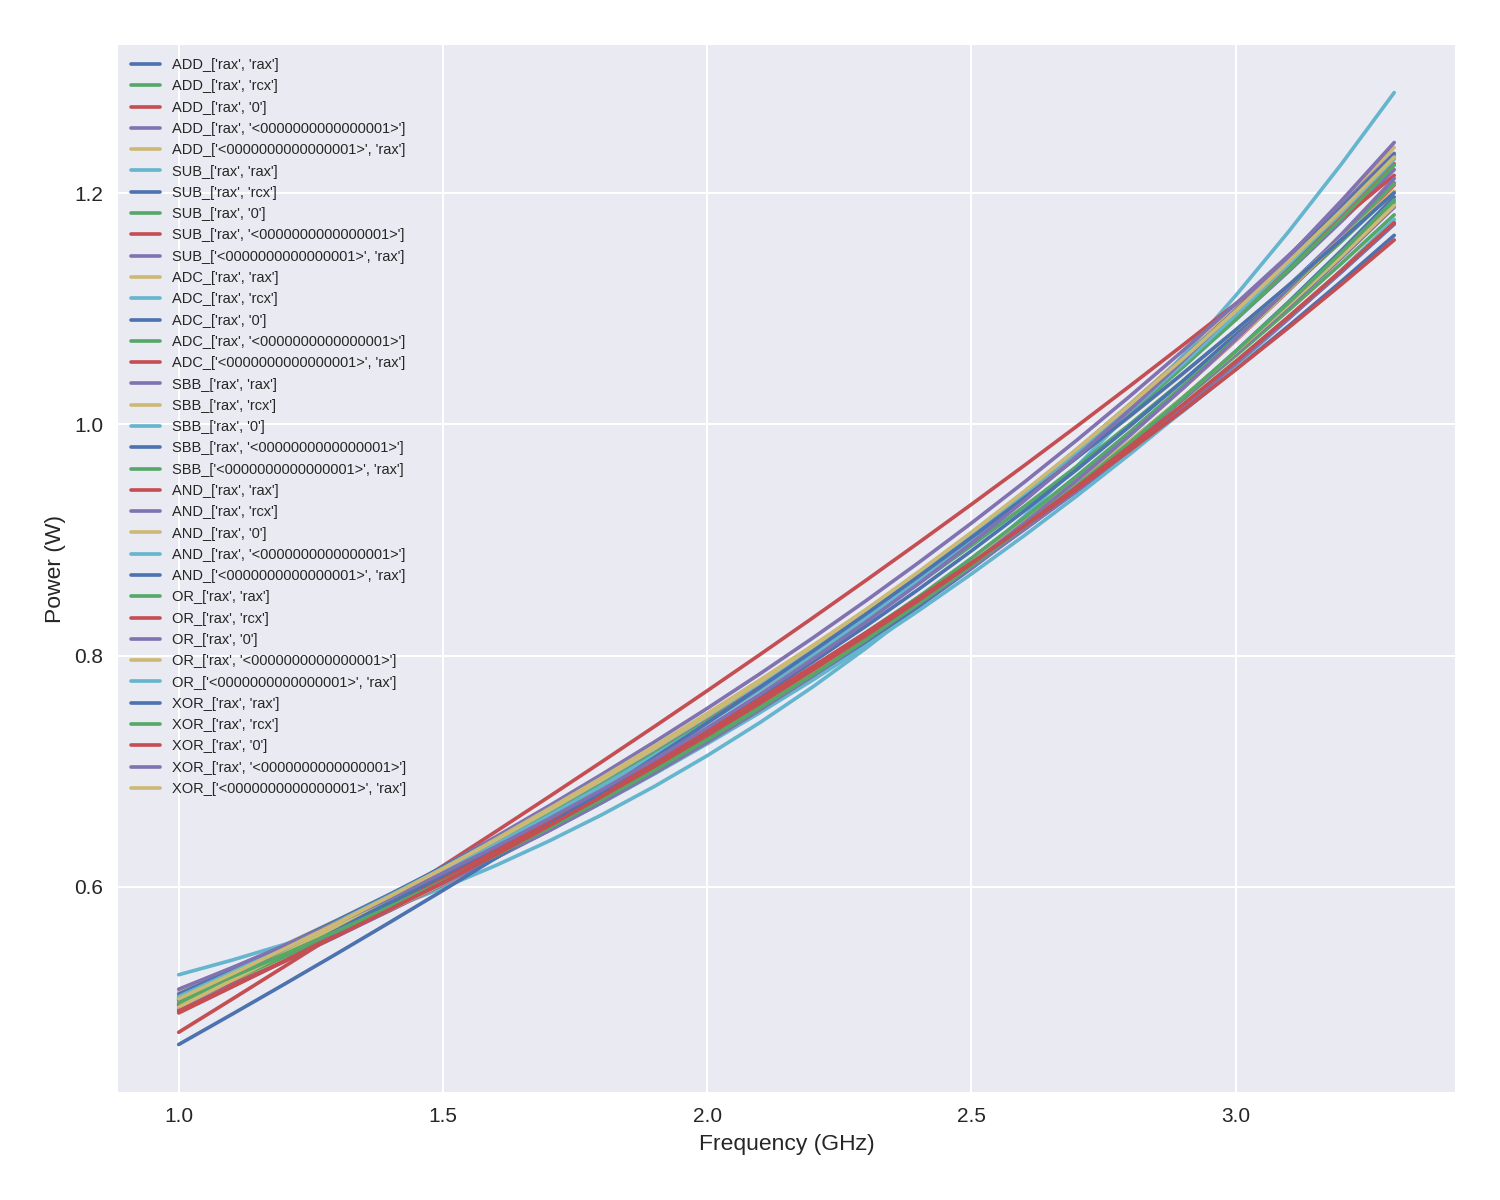
\includegraphics[width=\textwidth]{experiments/figures/inst_pw_args.png}
	\caption{Instructions power draw by argument}
	\label{fig:experiment_pw2}
\end{figure}

\section{Tracing application methods}

\begin{outline}
	\1 Linux ptrace
		\2 Breakpoint on each instruction	
	\1 Intel pin
		\2 JIT
		\2 Not open source
	\1 qemu user
		\2 TCG accelerator (transform target to host instruction) similar to JIT
		\2 Partial emulation
\end{outline}

We choose the less intrusive and open-source alternative qemu user, with an small modificaion we are able to trace an application instructions. Generating an table as follows:


\begin{table}[H]
	\centering
	\begin{tabular}{|c|c|c|}
		\hline
		opcode         & mnemonic & args                          \\ \hline
		48 89 e7       & movq     & \%rsp, \%rdi\textbackslash{}n \\ \hline
		48 89 e7       & movq     & \%rsp, \%rdi\textbackslash{}n \\ \hline
		e8 08 0e 00 00 & callq    & 0x4000a24ea0\textbackslash{}n \\ \hline
		55             & pushq    & \%rbp\textbackslash{}n        \\ \hline
		48 89 e5       & movq     & \%rsp, \%rbp\textbackslash{}n \\ \hline
		41 57          & pushq    & \%r15\textbackslash{}n        \\ \hline
		41 56          & pushq    & \%r14\textbackslash{}n        \\ \hline
		41 55          & pushq    & \%r13\textbackslash{}n        \\ \hline
		& \vdots & \\ \hline
	\end{tabular}
\end{table}


\section{CPU load}

\begin{figure}[H]
	\centering
	\begin{subfigure}[b]{0.45\textwidth}
		\centering
		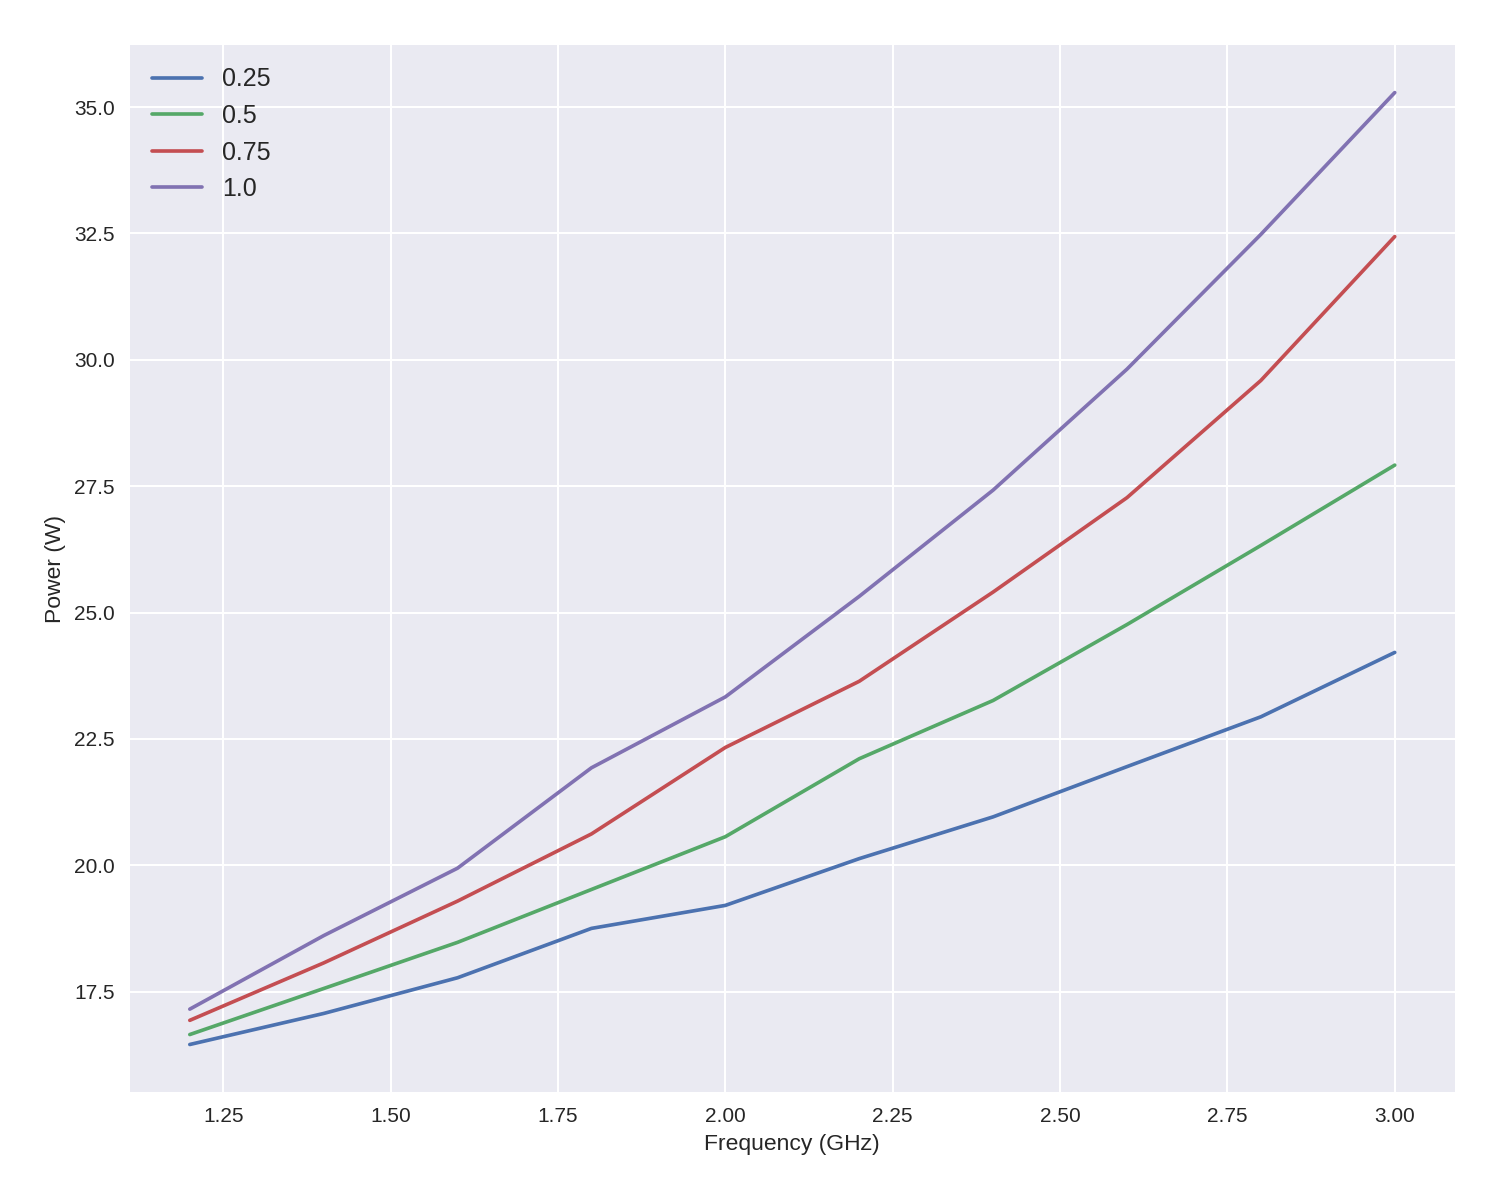
\includegraphics[width=1\columnwidth]{experiments/figures/pw_freq_load.png}
		\caption{Instructions power draw varing CPU load}
		\label{fig:experiment_pw_load}
	\end{subfigure}
	%
	\begin{subfigure}[b]{0.45\textwidth}
		\centering
		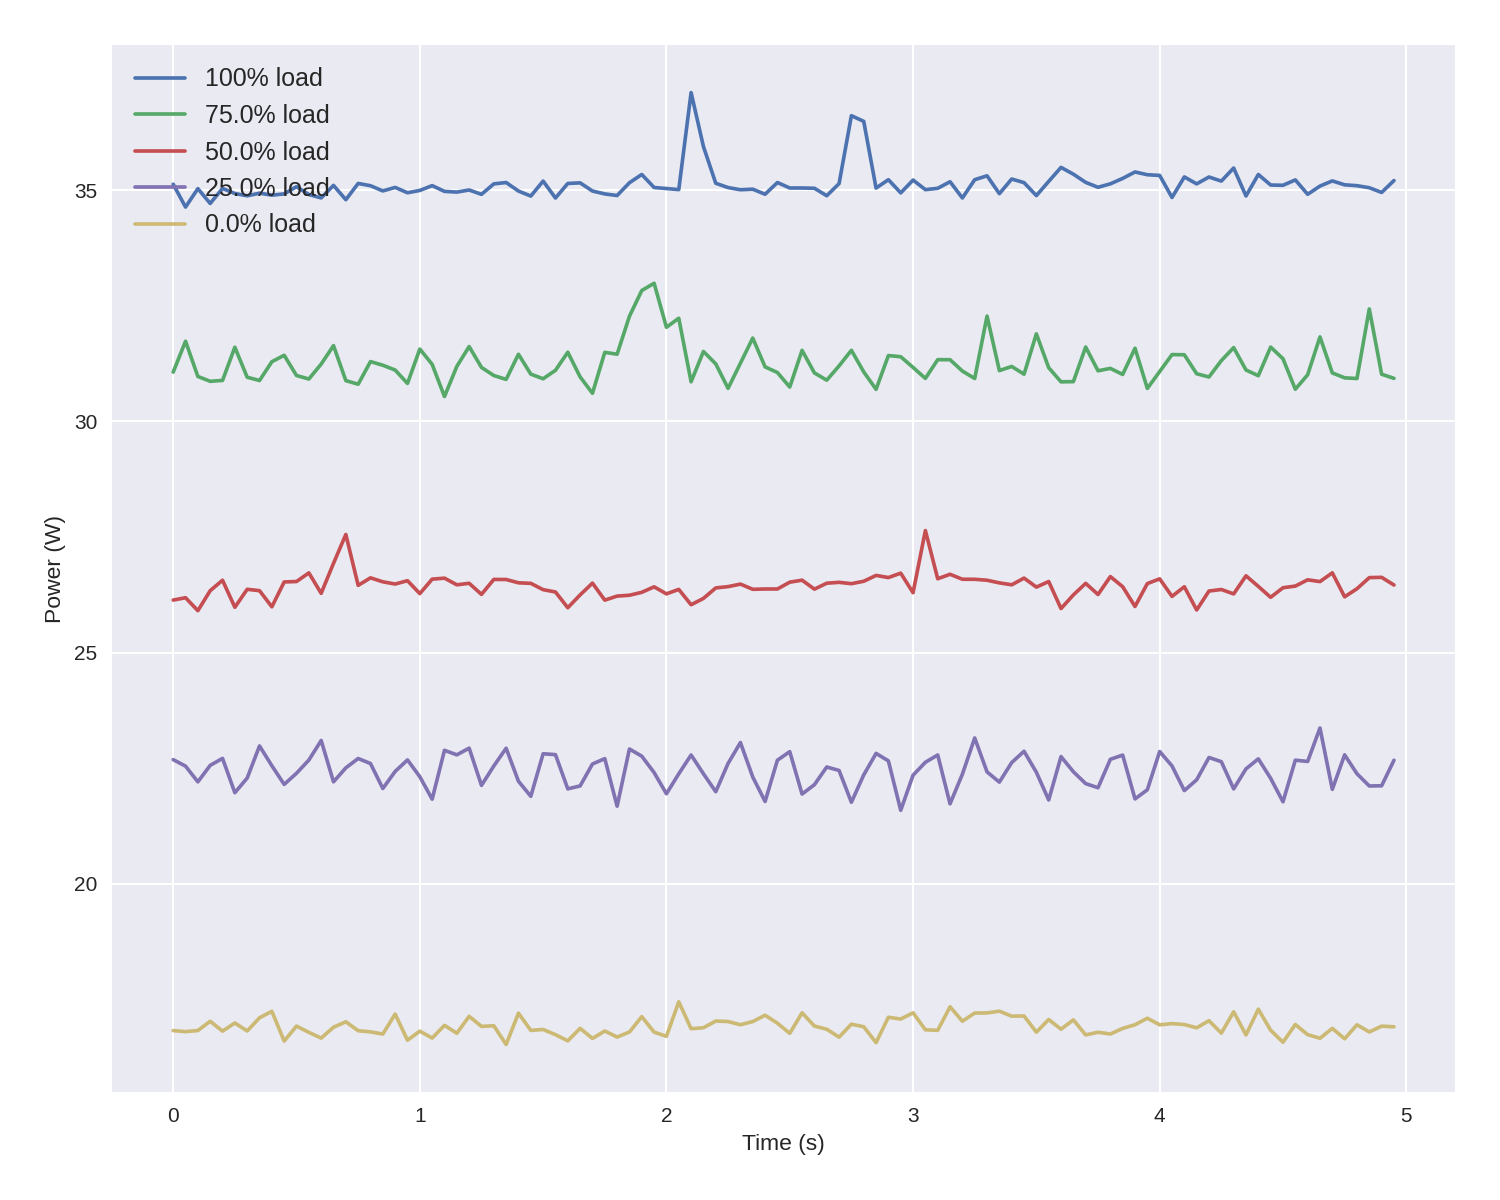
\includegraphics[width=1\columnwidth]{experiments/figures/pw_load.png}
		\caption{Instructions power draw varing CPU load}
		\label{fig:experiment_pw_load}
	\end{subfigure}
\end{figure}